\documentclass[twoside]{book}

% Packages required by doxygen
\usepackage{calc}
\usepackage{doxygen}
\usepackage{graphicx}
\usepackage[utf8]{inputenc}
\usepackage{makeidx}
\usepackage{multicol}
\usepackage{multirow}
\usepackage{textcomp}
\usepackage[table]{xcolor}

% Font selection
\usepackage[T1]{fontenc}
\usepackage{mathptmx}
\usepackage[scaled=.90]{helvet}
\usepackage{courier}
\usepackage{amssymb}
\usepackage{sectsty}
\renewcommand{\familydefault}{\sfdefault}
\allsectionsfont{%
  \fontseries{bc}\selectfont%
  \color{darkgray}%
}
\renewcommand{\DoxyLabelFont}{%
  \fontseries{bc}\selectfont%
  \color{darkgray}%
}

% Page & text layout
\usepackage{geometry}
\geometry{%
  a4paper,%
  top=2.5cm,%
  bottom=2.5cm,%
  left=2.5cm,%
  right=2.5cm%
}
\tolerance=750
\hfuzz=15pt
\hbadness=750
\setlength{\emergencystretch}{15pt}
\setlength{\parindent}{0cm}
\setlength{\parskip}{0.2cm}
\makeatletter
\renewcommand{\paragraph}{%
  \@startsection{paragraph}{4}{0ex}{-1.0ex}{1.0ex}{%
    \normalfont\normalsize\bfseries\SS@parafont%
  }%
}
\renewcommand{\subparagraph}{%
  \@startsection{subparagraph}{5}{0ex}{-1.0ex}{1.0ex}{%
    \normalfont\normalsize\bfseries\SS@subparafont%
  }%
}
\makeatother

% Headers & footers
\usepackage{fancyhdr}
\pagestyle{fancyplain}
\fancyhead[LE]{\fancyplain{}{\bfseries\thepage}}
\fancyhead[CE]{\fancyplain{}{}}
\fancyhead[RE]{\fancyplain{}{\bfseries\leftmark}}
\fancyhead[LO]{\fancyplain{}{\bfseries\rightmark}}
\fancyhead[CO]{\fancyplain{}{}}
\fancyhead[RO]{\fancyplain{}{\bfseries\thepage}}
\fancyfoot[LE]{\fancyplain{}{}}
\fancyfoot[CE]{\fancyplain{}{}}
\fancyfoot[RE]{\fancyplain{}{\bfseries\scriptsize Generated on Wed Jun 22 2016 15\-:26\-:28 for C\-A\-P\-I\-T\-A\-L by Doxygen }}
\fancyfoot[LO]{\fancyplain{}{\bfseries\scriptsize Generated on Wed Jun 22 2016 15\-:26\-:28 for C\-A\-P\-I\-T\-A\-L by Doxygen }}
\fancyfoot[CO]{\fancyplain{}{}}
\fancyfoot[RO]{\fancyplain{}{}}
\renewcommand{\footrulewidth}{0.4pt}
\renewcommand{\chaptermark}[1]{%
  \markboth{#1}{}%
}
\renewcommand{\sectionmark}[1]{%
  \markright{\thesection\ #1}%
}

% Indices & bibliography
\usepackage{natbib}
\usepackage[titles]{tocloft}
\setcounter{tocdepth}{3}
\setcounter{secnumdepth}{5}
\makeindex

% Hyperlinks (required, but should be loaded last)
\usepackage{ifpdf}
\ifpdf
  \usepackage[pdftex,pagebackref=true]{hyperref}
\else
  \usepackage[ps2pdf,pagebackref=true]{hyperref}
\fi
\hypersetup{%
  colorlinks=true,%
  linkcolor=blue,%
  citecolor=blue,%
  unicode%
}

% Custom commands
\newcommand{\clearemptydoublepage}{%
  \newpage{\pagestyle{empty}\cleardoublepage}%
}


%===== C O N T E N T S =====

\begin{document}

% Titlepage & ToC
\hypersetup{pageanchor=false}
\pagenumbering{roman}
\begin{titlepage}
\vspace*{7cm}
\begin{center}%
{\Large C\-A\-P\-I\-T\-A\-L \\[1ex]\large 1.\-0.\-0 }\\
\vspace*{1cm}
{\large Generated by Doxygen 1.8.6}\\
\vspace*{0.5cm}
{\small Wed Jun 22 2016 15:26:28}\\
\end{center}
\end{titlepage}
\clearemptydoublepage
\tableofcontents
\clearemptydoublepage
\pagenumbering{arabic}
\hypersetup{pageanchor=true}

%--- Begin generated contents ---
\chapter{Hierarchical Index}
\section{Class Hierarchy}
This inheritance list is sorted roughly, but not completely, alphabetically\-:\begin{DoxyCompactList}
\item \contentsline{section}{\-\_\-cvalue}{\pageref{union__cvalue}}{}
\item \contentsline{section}{Capital\-Function}{\pageref{classCapitalFunction}}{}
\item \contentsline{section}{Capital\-Value}{\pageref{classCapitalValue}}{}
\item \contentsline{section}{message\-\_\-header}{\pageref{structmessage__header}}{}
\begin{DoxyCompactList}
\item \contentsline{section}{msg\-\_\-advertise}{\pageref{structmsg__advertise}}{}
\item \contentsline{section}{msg\-\_\-connack}{\pageref{structmsg__connack}}{}
\item \contentsline{section}{msg\-\_\-connect}{\pageref{structmsg__connect}}{}
\item \contentsline{section}{msg\-\_\-devreg}{\pageref{structmsg__devreg}}{}
\item \contentsline{section}{msg\-\_\-devregack}{\pageref{structmsg__devregack}}{}
\item \contentsline{section}{msg\-\_\-disconnect}{\pageref{structmsg__disconnect}}{}
\item \contentsline{section}{msg\-\_\-gwinfo}{\pageref{structmsg__gwinfo}}{}
\item \contentsline{section}{msg\-\_\-pingreq}{\pageref{structmsg__pingreq}}{}
\item \contentsline{section}{msg\-\_\-puback}{\pageref{structmsg__puback}}{}
\item \contentsline{section}{msg\-\_\-publish}{\pageref{structmsg__publish}}{}
\item \contentsline{section}{msg\-\_\-pubqos2}{\pageref{structmsg__pubqos2}}{}
\item \contentsline{section}{msg\-\_\-regack}{\pageref{structmsg__regack}}{}
\item \contentsline{section}{msg\-\_\-register}{\pageref{structmsg__register}}{}
\item \contentsline{section}{msg\-\_\-searchgw}{\pageref{structmsg__searchgw}}{}
\item \contentsline{section}{msg\-\_\-suback}{\pageref{structmsg__suback}}{}
\item \contentsline{section}{msg\-\_\-subscribe}{\pageref{structmsg__subscribe}}{}
\item \contentsline{section}{msg\-\_\-unsuback}{\pageref{structmsg__unsuback}}{}
\item \contentsline{section}{msg\-\_\-unsubscribe}{\pageref{structmsg__unsubscribe}}{}
\item \contentsline{section}{msg\-\_\-willmsg}{\pageref{structmsg__willmsg}}{}
\item \contentsline{section}{msg\-\_\-willmsgresp}{\pageref{structmsg__willmsgresp}}{}
\item \contentsline{section}{msg\-\_\-willtopic}{\pageref{structmsg__willtopic}}{}
\item \contentsline{section}{msg\-\_\-willtopicresp}{\pageref{structmsg__willtopicresp}}{}
\end{DoxyCompactList}
\item \contentsline{section}{Thing\-Client}{\pageref{classThingClient}}{}
\end{DoxyCompactList}

\chapter{Class Index}
\section{Class List}
Here are the classes, structs, unions and interfaces with brief descriptions\-:\begin{DoxyCompactList}
\item\contentsline{section}{\hyperlink{union__cvalue}{\-\_\-cvalue} }{\pageref{union__cvalue}}{}
\item\contentsline{section}{\hyperlink{classCapitalFunction}{Capital\-Function} \\*A class for handling various \char`\"{}function\char`\"{} types }{\pageref{classCapitalFunction}}{}
\item\contentsline{section}{\hyperlink{classCapitalValue}{Capital\-Value} \\*A class for handling various \char`\"{}value\char`\"{} types }{\pageref{classCapitalValue}}{}
\item\contentsline{section}{\hyperlink{structmessage__header}{message\-\_\-header} }{\pageref{structmessage__header}}{}
\item\contentsline{section}{\hyperlink{structmsg__advertise}{msg\-\_\-advertise} }{\pageref{structmsg__advertise}}{}
\item\contentsline{section}{\hyperlink{structmsg__connack}{msg\-\_\-connack} }{\pageref{structmsg__connack}}{}
\item\contentsline{section}{\hyperlink{structmsg__connect}{msg\-\_\-connect} }{\pageref{structmsg__connect}}{}
\item\contentsline{section}{\hyperlink{structmsg__devreg}{msg\-\_\-devreg} }{\pageref{structmsg__devreg}}{}
\item\contentsline{section}{\hyperlink{structmsg__devregack}{msg\-\_\-devregack} }{\pageref{structmsg__devregack}}{}
\item\contentsline{section}{\hyperlink{structmsg__disconnect}{msg\-\_\-disconnect} }{\pageref{structmsg__disconnect}}{}
\item\contentsline{section}{\hyperlink{structmsg__gwinfo}{msg\-\_\-gwinfo} }{\pageref{structmsg__gwinfo}}{}
\item\contentsline{section}{\hyperlink{structmsg__pingreq}{msg\-\_\-pingreq} }{\pageref{structmsg__pingreq}}{}
\item\contentsline{section}{\hyperlink{structmsg__puback}{msg\-\_\-puback} }{\pageref{structmsg__puback}}{}
\item\contentsline{section}{\hyperlink{structmsg__publish}{msg\-\_\-publish} }{\pageref{structmsg__publish}}{}
\item\contentsline{section}{\hyperlink{structmsg__pubqos2}{msg\-\_\-pubqos2} }{\pageref{structmsg__pubqos2}}{}
\item\contentsline{section}{\hyperlink{structmsg__regack}{msg\-\_\-regack} }{\pageref{structmsg__regack}}{}
\item\contentsline{section}{\hyperlink{structmsg__register}{msg\-\_\-register} }{\pageref{structmsg__register}}{}
\item\contentsline{section}{\hyperlink{structmsg__searchgw}{msg\-\_\-searchgw} }{\pageref{structmsg__searchgw}}{}
\item\contentsline{section}{\hyperlink{structmsg__suback}{msg\-\_\-suback} }{\pageref{structmsg__suback}}{}
\item\contentsline{section}{\hyperlink{structmsg__subscribe}{msg\-\_\-subscribe} }{\pageref{structmsg__subscribe}}{}
\item\contentsline{section}{\hyperlink{structmsg__unsuback}{msg\-\_\-unsuback} }{\pageref{structmsg__unsuback}}{}
\item\contentsline{section}{\hyperlink{structmsg__unsubscribe}{msg\-\_\-unsubscribe} }{\pageref{structmsg__unsubscribe}}{}
\item\contentsline{section}{\hyperlink{structmsg__willmsg}{msg\-\_\-willmsg} }{\pageref{structmsg__willmsg}}{}
\item\contentsline{section}{\hyperlink{structmsg__willmsgresp}{msg\-\_\-willmsgresp} }{\pageref{structmsg__willmsgresp}}{}
\item\contentsline{section}{\hyperlink{structmsg__willtopic}{msg\-\_\-willtopic} }{\pageref{structmsg__willtopic}}{}
\item\contentsline{section}{\hyperlink{structmsg__willtopicresp}{msg\-\_\-willtopicresp} }{\pageref{structmsg__willtopicresp}}{}
\item\contentsline{section}{\hyperlink{classThingClient}{Thing\-Client} \\*A class for communication between thing and gateway }{\pageref{classThingClient}}{}
\end{DoxyCompactList}

\chapter{File Index}
\section{File List}
Here is a list of all documented files with brief descriptions\-:\begin{DoxyCompactList}
\item\contentsline{section}{\hyperlink{thing__client_8h}{thing\-\_\-client.\-h} \\*Class Value, Function, Client included }{\pageref{thing__client_8h}}{}
\item\contentsline{section}{\hyperlink{thing__defines_8h}{thing\-\_\-defines.\-h} \\*Define macros, default enums and types }{\pageref{thing__defines_8h}}{}
\end{DoxyCompactList}

\chapter{Class Documentation}
\hypertarget{union__cvalue}{\section{\-\_\-cvalue Union Reference}
\label{union__cvalue}\index{\-\_\-cvalue@{\-\_\-cvalue}}
}
\subsection*{Public Attributes}
\begin{DoxyCompactItemize}
\item 
\hypertarget{union__cvalue_aa314ceeb89f39b472259ae4c6d8a084e}{double {\bfseries double\-\_\-}}\label{union__cvalue_aa314ceeb89f39b472259ae4c6d8a084e}

\item 
\hypertarget{union__cvalue_a9e76d8e55278ba6c505ff6426458aa0e}{int {\bfseries int\-\_\-}}\label{union__cvalue_a9e76d8e55278ba6c505ff6426458aa0e}

\end{DoxyCompactItemize}


The documentation for this union was generated from the following file\-:\begin{DoxyCompactItemize}
\item 
\hyperlink{thing__defines_8h}{thing\-\_\-defines.\-h}\end{DoxyCompactItemize}

\hypertarget{classCapitalFunction}{\section{Capital\-Function Class Reference}
\label{classCapitalFunction}\index{Capital\-Function@{Capital\-Function}}
}


A class for handling various \char`\"{}function\char`\"{} types.  




{\ttfamily \#include $<$thing\-\_\-client.\-h$>$}

\subsection*{Public Member Functions}
\begin{DoxyCompactItemize}
\item 
\hyperlink{classCapitalFunction_aa2b99fd29c519f475e5fe06eac460f9a}{$\sim$\-Capital\-Function} ()
\item 
void \hyperlink{classCapitalFunction_a8f5f8a9b32b18c806bb9b33dd355ec86}{set\-\_\-name} (const char $\ast$\hyperlink{classCapitalFunction_af492834dfd92eb02e0c0bf915fc58755}{name})
\item 
char $\ast$ \hyperlink{classCapitalFunction_af492834dfd92eb02e0c0bf915fc58755}{name} ()
\item 
void $\ast$ \hyperlink{classCapitalFunction_a402a1c3915165656da3fbf1636777da0}{function} ()
\end{DoxyCompactItemize}
\begin{Indent}{\bf incomplete Constructors}\par
{\em Name and function must be set. Also, if the argument type of the function is integer, double, or const char$\ast$, min and max must be set. (In the case of const char$\ast$, min and max indicates minimum length and maximum length of the array.)


\begin{DoxyParams}{Parameters}
{\em ($\ast$function)} & means the function pointer \\
\hline
{\em min} & means the minimum argument value of the function \\
\hline
{\em max} & means the maximum argument value of the function \\
\hline
\end{DoxyParams}
}\begin{DoxyCompactItemize}
\item 
\hyperlink{classCapitalFunction_a51342fe3645d8874ed4a3a7074ec043c}{Capital\-Function} ()
\item 
\hypertarget{classCapitalFunction_aef6043f114f3266a3303dea974f69ce9}{{\bfseries Capital\-Function} (void($\ast$func)(void))}\label{classCapitalFunction_aef6043f114f3266a3303dea974f69ce9}

\item 
\hypertarget{classCapitalFunction_a9fe7f4522d611a4b9de22dd57459281f}{{\bfseries Capital\-Function} (void($\ast$func)(int arg))}\label{classCapitalFunction_a9fe7f4522d611a4b9de22dd57459281f}

\item 
\hypertarget{classCapitalFunction_a00aacf178c2d0283ed5029e43216fd5e}{{\bfseries Capital\-Function} (void($\ast$func)(double arg))}\label{classCapitalFunction_a00aacf178c2d0283ed5029e43216fd5e}

\item 
\hypertarget{classCapitalFunction_a7ed72e105935ec87fad0b7bc1f4c324b}{{\bfseries Capital\-Function} (void($\ast$func)(bool arg))}\label{classCapitalFunction_a7ed72e105935ec87fad0b7bc1f4c324b}

\item 
\hypertarget{classCapitalFunction_a812504f8e7913c1b733f12a2e9c3a9ac}{{\bfseries Capital\-Function} (void($\ast$func)(int arg), int min, int max)}\label{classCapitalFunction_a812504f8e7913c1b733f12a2e9c3a9ac}

\item 
\hypertarget{classCapitalFunction_acdb268f1f4e45fc2c8360ba896f14ab6}{{\bfseries Capital\-Function} (void($\ast$func)(double arg), double min, double max)}\label{classCapitalFunction_acdb268f1f4e45fc2c8360ba896f14ab6}

\end{DoxyCompactItemize}
\end{Indent}
\begin{Indent}{\bf complete Constructors}\par
{\em while using 4 Constructors below, it can be added to the Client without any function calls


\begin{DoxyParams}{Parameters}
{\em name} & means the name of the function \\
\hline
\end{DoxyParams}
}\begin{DoxyCompactItemize}
\item 
\hyperlink{classCapitalFunction_a89f0d476564dabdc3a5a4eefd75c0110}{Capital\-Function} (const char $\ast$\hyperlink{classCapitalFunction_af492834dfd92eb02e0c0bf915fc58755}{name}, void($\ast$func)(void))
\item 
\hyperlink{classCapitalFunction_a4b6121b145df9833019c53dde7bad362}{Capital\-Function} (const char $\ast$\hyperlink{classCapitalFunction_af492834dfd92eb02e0c0bf915fc58755}{name}, void($\ast$func)(bool arg))
\item 
\hyperlink{classCapitalFunction_a6eadfbcd622f9cb3c5d5fca694042379}{Capital\-Function} (const char $\ast$\hyperlink{classCapitalFunction_af492834dfd92eb02e0c0bf915fc58755}{name}, void($\ast$func)(int arg), int min, int max)
\item 
\hyperlink{classCapitalFunction_ad15d886cbb971ce64b0131964df5fdb0}{Capital\-Function} (const char $\ast$\hyperlink{classCapitalFunction_af492834dfd92eb02e0c0bf915fc58755}{name}, void($\ast$func)(double arg), double min, double max)
\end{DoxyCompactItemize}
\end{Indent}
\begin{Indent}{\bf set function}\par
{\em set function pointer }\begin{DoxyCompactItemize}
\item 
void \hyperlink{classCapitalFunction_a3548899a70e6c0ad633016f2c7154504}{set\-\_\-function} (void($\ast$func)(void))
\item 
void \hyperlink{classCapitalFunction_a2b27b8f4aea08075b102c102be618205}{set\-\_\-function} (void($\ast$func)(int arg))
\item 
void \hyperlink{classCapitalFunction_ab8a52f2a27c3773cd8d10b3e0136252f}{set\-\_\-function} (void($\ast$func)(double arg))
\item 
void \hyperlink{classCapitalFunction_aad7892103b04ce726a4b5d6052383df2}{set\-\_\-function} (void($\ast$func)(bool arg))
\end{DoxyCompactItemize}
\end{Indent}
\begin{Indent}{\bf set minmax}\par
{\em set the minimum value or maximum of the value }\begin{DoxyCompactItemize}
\item 
void \hyperlink{classCapitalFunction_ae0d414289f9e6b97d408a3fd56818d62}{set\-\_\-min} (const int min)
\item 
void \hyperlink{classCapitalFunction_a90cc64dbc33810044903663f43b6281a}{set\-\_\-min} (const double min)
\item 
void \hyperlink{classCapitalFunction_a18968f5530879cbbeee6f0ed5b4e5b06}{set\-\_\-max} (const int max)
\item 
void \hyperlink{classCapitalFunction_ab30fe1096d179553407e1f393e2b3bb3}{set\-\_\-max} (const double max)
\end{DoxyCompactItemize}
\end{Indent}
\subsection*{Execute}
\label{_amgrp40cd014b7b6251e3a22e6a45a73a64e1}%
Execute the function with argument 
\begin{DoxyParams}{Parameters}
{\em arg} & the input argument of the function \\
\hline
\end{DoxyParams}
\begin{DoxyCompactItemize}
\item 
void \hyperlink{classCapitalFunction_a186d9595b28182ab66a6dc852e886b51}{Execute} (void) const 
\item 
int \hyperlink{classCapitalFunction_ab2e4ab2da79f3a1ddd35a03d83b01940}{Execute} (int arg) const 
\item 
int \hyperlink{classCapitalFunction_acec9c2031c60781057076a75038c506b}{Execute} (double arg) const 
\item 
void \hyperlink{classCapitalFunction_a87f340ed78a0a302aac69252987a7eb6}{Execute} (bool arg) const 
\item 
void \hyperlink{classCapitalFunction_ac8c2cc35ea735b4197cf080828b708d3}{Get\-Information} (char $\ast$buffer)
\item 
uint16\-\_\-t \hyperlink{classCapitalFunction_aed6d3adf21ec01f78ef7fbc78b7db072}{set\-\_\-id\-\_\-1003} (uint16\-\_\-t \hyperlink{classCapitalFunction_a15bb55ddfec1ad1c3c21fe1493e00f33}{id\-\_\-1003})
\item 
uint16\-\_\-t \hyperlink{classCapitalFunction_a15bb55ddfec1ad1c3c21fe1493e00f33}{id\-\_\-1003} ()
\item 
uint16\-\_\-t \hyperlink{classCapitalFunction_a645a79adaa1676f7bc7f7be4033d87ae}{set\-\_\-id\-\_\-2004} (uint16\-\_\-t \hyperlink{classCapitalFunction_a7eef4dc83c5fc8529ceb30372316af55}{id\-\_\-2004})
\item 
uint16\-\_\-t \hyperlink{classCapitalFunction_a7eef4dc83c5fc8529ceb30372316af55}{id\-\_\-2004} ()
\item 
\hypertarget{classCapitalFunction_a5fb54b80f92a1620d1e3b2f74a7b260e}{Cap\-Type {\bfseries function\-\_\-classifier} (void)}\label{classCapitalFunction_a5fb54b80f92a1620d1e3b2f74a7b260e}

\end{DoxyCompactItemize}


\subsection{Detailed Description}
A class for handling various \char`\"{}function\char`\"{} types. 

A programmer can add Functions to the Supervisor by using this class. void f(void $\vert$ int $\vert$ double $\vert$ bool) -\/ only 4 types can be handled 

\subsection{Constructor \& Destructor Documentation}
\hypertarget{classCapitalFunction_a51342fe3645d8874ed4a3a7074ec043c}{\index{Capital\-Function@{Capital\-Function}!Capital\-Function@{Capital\-Function}}
\index{Capital\-Function@{Capital\-Function}!CapitalFunction@{Capital\-Function}}
\subsubsection[{Capital\-Function}]{\setlength{\rightskip}{0pt plus 5cm}Capital\-Function\-::\-Capital\-Function (
\begin{DoxyParamCaption}
{}
\end{DoxyParamCaption}
)}}\label{classCapitalFunction_a51342fe3645d8874ed4a3a7074ec043c}
default constructor \hypertarget{classCapitalFunction_a89f0d476564dabdc3a5a4eefd75c0110}{\index{Capital\-Function@{Capital\-Function}!Capital\-Function@{Capital\-Function}}
\index{Capital\-Function@{Capital\-Function}!CapitalFunction@{Capital\-Function}}
\subsubsection[{Capital\-Function}]{\setlength{\rightskip}{0pt plus 5cm}Capital\-Function\-::\-Capital\-Function (
\begin{DoxyParamCaption}
\item[{const char $\ast$}]{name, }
\item[{void($\ast$)(void)}]{func}
\end{DoxyParamCaption}
)}}\label{classCapitalFunction_a89f0d476564dabdc3a5a4eefd75c0110}
constructor for void function 
\begin{DoxyParams}{Parameters}
{\em name} & means the name of the function \\
\hline
\end{DoxyParams}
\hypertarget{classCapitalFunction_a4b6121b145df9833019c53dde7bad362}{\index{Capital\-Function@{Capital\-Function}!Capital\-Function@{Capital\-Function}}
\index{Capital\-Function@{Capital\-Function}!CapitalFunction@{Capital\-Function}}
\subsubsection[{Capital\-Function}]{\setlength{\rightskip}{0pt plus 5cm}Capital\-Function\-::\-Capital\-Function (
\begin{DoxyParamCaption}
\item[{const char $\ast$}]{name, }
\item[{void($\ast$)(bool arg)}]{func}
\end{DoxyParamCaption}
)}}\label{classCapitalFunction_a4b6121b145df9833019c53dde7bad362}
constructor for bool-\/argument function 
\begin{DoxyParams}{Parameters}
{\em name} & means the name of the function \\
\hline
\end{DoxyParams}
\hypertarget{classCapitalFunction_a6eadfbcd622f9cb3c5d5fca694042379}{\index{Capital\-Function@{Capital\-Function}!Capital\-Function@{Capital\-Function}}
\index{Capital\-Function@{Capital\-Function}!CapitalFunction@{Capital\-Function}}
\subsubsection[{Capital\-Function}]{\setlength{\rightskip}{0pt plus 5cm}Capital\-Function\-::\-Capital\-Function (
\begin{DoxyParamCaption}
\item[{const char $\ast$}]{name, }
\item[{void($\ast$)(int arg)}]{func, }
\item[{int}]{min, }
\item[{int}]{max}
\end{DoxyParamCaption}
)}}\label{classCapitalFunction_a6eadfbcd622f9cb3c5d5fca694042379}
constructor for integer-\/argument function 
\begin{DoxyParams}{Parameters}
{\em name} & means the name of the function \\
\hline
{\em min} & represents minimum value of the argument \\
\hline
{\em max} & represents maximum value of the argument \\
\hline
\end{DoxyParams}
\hypertarget{classCapitalFunction_ad15d886cbb971ce64b0131964df5fdb0}{\index{Capital\-Function@{Capital\-Function}!Capital\-Function@{Capital\-Function}}
\index{Capital\-Function@{Capital\-Function}!CapitalFunction@{Capital\-Function}}
\subsubsection[{Capital\-Function}]{\setlength{\rightskip}{0pt plus 5cm}Capital\-Function\-::\-Capital\-Function (
\begin{DoxyParamCaption}
\item[{const char $\ast$}]{name, }
\item[{void($\ast$)(double arg)}]{func, }
\item[{double}]{min, }
\item[{double}]{max}
\end{DoxyParamCaption}
)}}\label{classCapitalFunction_ad15d886cbb971ce64b0131964df5fdb0}
constructor for double-\/argument function 
\begin{DoxyParams}{Parameters}
{\em name} & means the name of the function \\
\hline
{\em min} & represents minimum value of the argument \\
\hline
{\em max} & represents maximum value of the argument \\
\hline
\end{DoxyParams}
\hypertarget{classCapitalFunction_aa2b99fd29c519f475e5fe06eac460f9a}{\index{Capital\-Function@{Capital\-Function}!$\sim$\-Capital\-Function@{$\sim$\-Capital\-Function}}
\index{$\sim$\-Capital\-Function@{$\sim$\-Capital\-Function}!CapitalFunction@{Capital\-Function}}
\subsubsection[{$\sim$\-Capital\-Function}]{\setlength{\rightskip}{0pt plus 5cm}Capital\-Function\-::$\sim$\-Capital\-Function (
\begin{DoxyParamCaption}
{}
\end{DoxyParamCaption}
)}}\label{classCapitalFunction_aa2b99fd29c519f475e5fe06eac460f9a}
A destructor 

\subsection{Member Function Documentation}
\hypertarget{classCapitalFunction_a186d9595b28182ab66a6dc852e886b51}{\index{Capital\-Function@{Capital\-Function}!Execute@{Execute}}
\index{Execute@{Execute}!CapitalFunction@{Capital\-Function}}
\subsubsection[{Execute}]{\setlength{\rightskip}{0pt plus 5cm}void Capital\-Function\-::\-Execute (
\begin{DoxyParamCaption}
\item[{void}]{}
\end{DoxyParamCaption}
) const}}\label{classCapitalFunction_a186d9595b28182ab66a6dc852e886b51}
Execute void function (it occurs error when it is not a void function) \hypertarget{classCapitalFunction_ab2e4ab2da79f3a1ddd35a03d83b01940}{\index{Capital\-Function@{Capital\-Function}!Execute@{Execute}}
\index{Execute@{Execute}!CapitalFunction@{Capital\-Function}}
\subsubsection[{Execute}]{\setlength{\rightskip}{0pt plus 5cm}int Capital\-Function\-::\-Execute (
\begin{DoxyParamCaption}
\item[{int}]{arg}
\end{DoxyParamCaption}
) const}}\label{classCapitalFunction_ab2e4ab2da79f3a1ddd35a03d83b01940}
Execute integer function with argument (it occurs error when argument does not matches) it returns error code by comparing min, max and argument \hypertarget{classCapitalFunction_acec9c2031c60781057076a75038c506b}{\index{Capital\-Function@{Capital\-Function}!Execute@{Execute}}
\index{Execute@{Execute}!CapitalFunction@{Capital\-Function}}
\subsubsection[{Execute}]{\setlength{\rightskip}{0pt plus 5cm}int Capital\-Function\-::\-Execute (
\begin{DoxyParamCaption}
\item[{double}]{arg}
\end{DoxyParamCaption}
) const}}\label{classCapitalFunction_acec9c2031c60781057076a75038c506b}
Execute double function with argument (it occurs error when argument does not matches) it returns error code by comparing min, max and argument \hypertarget{classCapitalFunction_a87f340ed78a0a302aac69252987a7eb6}{\index{Capital\-Function@{Capital\-Function}!Execute@{Execute}}
\index{Execute@{Execute}!CapitalFunction@{Capital\-Function}}
\subsubsection[{Execute}]{\setlength{\rightskip}{0pt plus 5cm}void Capital\-Function\-::\-Execute (
\begin{DoxyParamCaption}
\item[{bool}]{arg}
\end{DoxyParamCaption}
) const}}\label{classCapitalFunction_a87f340ed78a0a302aac69252987a7eb6}
Execute bool function with argument (it occurs error when argument does not matches) \hypertarget{classCapitalFunction_a402a1c3915165656da3fbf1636777da0}{\index{Capital\-Function@{Capital\-Function}!function@{function}}
\index{function@{function}!CapitalFunction@{Capital\-Function}}
\subsubsection[{function}]{\setlength{\rightskip}{0pt plus 5cm}void$\ast$ Capital\-Function\-::function (
\begin{DoxyParamCaption}
{}
\end{DoxyParamCaption}
)}}\label{classCapitalFunction_a402a1c3915165656da3fbf1636777da0}
get pointer of the functione, it can be used with function\-\_\-classifier() \hypertarget{classCapitalFunction_ac8c2cc35ea735b4197cf080828b708d3}{\index{Capital\-Function@{Capital\-Function}!Get\-Information@{Get\-Information}}
\index{Get\-Information@{Get\-Information}!CapitalFunction@{Capital\-Function}}
\subsubsection[{Get\-Information}]{\setlength{\rightskip}{0pt plus 5cm}void Capital\-Function\-::\-Get\-Information (
\begin{DoxyParamCaption}
\item[{char $\ast$}]{buffer}
\end{DoxyParamCaption}
)}}\label{classCapitalFunction_ac8c2cc35ea735b4197cf080828b708d3}
Get a string that contains information of the function 
\begin{DoxyParams}{Parameters}
{\em buffer} & output buffer \\
\hline
\end{DoxyParams}
\hypertarget{classCapitalFunction_a15bb55ddfec1ad1c3c21fe1493e00f33}{\index{Capital\-Function@{Capital\-Function}!id\-\_\-1003@{id\-\_\-1003}}
\index{id\-\_\-1003@{id\-\_\-1003}!CapitalFunction@{Capital\-Function}}
\subsubsection[{id\-\_\-1003}]{\setlength{\rightskip}{0pt plus 5cm}uint16\-\_\-t Capital\-Function\-::id\-\_\-1003 (
\begin{DoxyParamCaption}
{}
\end{DoxyParamCaption}
)}}\label{classCapitalFunction_a15bb55ddfec1ad1c3c21fe1493e00f33}
get a registerd id of topic name from M\-T1003 \hypertarget{classCapitalFunction_a7eef4dc83c5fc8529ceb30372316af55}{\index{Capital\-Function@{Capital\-Function}!id\-\_\-2004@{id\-\_\-2004}}
\index{id\-\_\-2004@{id\-\_\-2004}!CapitalFunction@{Capital\-Function}}
\subsubsection[{id\-\_\-2004}]{\setlength{\rightskip}{0pt plus 5cm}uint16\-\_\-t Capital\-Function\-::id\-\_\-2004 (
\begin{DoxyParamCaption}
{}
\end{DoxyParamCaption}
)}}\label{classCapitalFunction_a7eef4dc83c5fc8529ceb30372316af55}
get a saved id\-\_\-2004 \hypertarget{classCapitalFunction_af492834dfd92eb02e0c0bf915fc58755}{\index{Capital\-Function@{Capital\-Function}!name@{name}}
\index{name@{name}!CapitalFunction@{Capital\-Function}}
\subsubsection[{name}]{\setlength{\rightskip}{0pt plus 5cm}char $\ast$ Capital\-Function\-::name (
\begin{DoxyParamCaption}
{}
\end{DoxyParamCaption}
)}}\label{classCapitalFunction_af492834dfd92eb02e0c0bf915fc58755}
get name's pointer of the function \hypertarget{classCapitalFunction_a3548899a70e6c0ad633016f2c7154504}{\index{Capital\-Function@{Capital\-Function}!set\-\_\-function@{set\-\_\-function}}
\index{set\-\_\-function@{set\-\_\-function}!CapitalFunction@{Capital\-Function}}
\subsubsection[{set\-\_\-function}]{\setlength{\rightskip}{0pt plus 5cm}void Capital\-Function\-::set\-\_\-function (
\begin{DoxyParamCaption}
\item[{void($\ast$)(void)}]{func}
\end{DoxyParamCaption}
)}}\label{classCapitalFunction_a3548899a70e6c0ad633016f2c7154504}
set void-\/argument function \hypertarget{classCapitalFunction_a2b27b8f4aea08075b102c102be618205}{\index{Capital\-Function@{Capital\-Function}!set\-\_\-function@{set\-\_\-function}}
\index{set\-\_\-function@{set\-\_\-function}!CapitalFunction@{Capital\-Function}}
\subsubsection[{set\-\_\-function}]{\setlength{\rightskip}{0pt plus 5cm}void Capital\-Function\-::set\-\_\-function (
\begin{DoxyParamCaption}
\item[{void($\ast$)(int arg)}]{func}
\end{DoxyParamCaption}
)}}\label{classCapitalFunction_a2b27b8f4aea08075b102c102be618205}
set integer-\/argument function \hypertarget{classCapitalFunction_ab8a52f2a27c3773cd8d10b3e0136252f}{\index{Capital\-Function@{Capital\-Function}!set\-\_\-function@{set\-\_\-function}}
\index{set\-\_\-function@{set\-\_\-function}!CapitalFunction@{Capital\-Function}}
\subsubsection[{set\-\_\-function}]{\setlength{\rightskip}{0pt plus 5cm}void Capital\-Function\-::set\-\_\-function (
\begin{DoxyParamCaption}
\item[{void($\ast$)(double arg)}]{func}
\end{DoxyParamCaption}
)}}\label{classCapitalFunction_ab8a52f2a27c3773cd8d10b3e0136252f}
set double-\/argument function \hypertarget{classCapitalFunction_aad7892103b04ce726a4b5d6052383df2}{\index{Capital\-Function@{Capital\-Function}!set\-\_\-function@{set\-\_\-function}}
\index{set\-\_\-function@{set\-\_\-function}!CapitalFunction@{Capital\-Function}}
\subsubsection[{set\-\_\-function}]{\setlength{\rightskip}{0pt plus 5cm}void Capital\-Function\-::set\-\_\-function (
\begin{DoxyParamCaption}
\item[{void($\ast$)(bool arg)}]{func}
\end{DoxyParamCaption}
)}}\label{classCapitalFunction_aad7892103b04ce726a4b5d6052383df2}
set bool-\/argument function \hypertarget{classCapitalFunction_aed6d3adf21ec01f78ef7fbc78b7db072}{\index{Capital\-Function@{Capital\-Function}!set\-\_\-id\-\_\-1003@{set\-\_\-id\-\_\-1003}}
\index{set\-\_\-id\-\_\-1003@{set\-\_\-id\-\_\-1003}!CapitalFunction@{Capital\-Function}}
\subsubsection[{set\-\_\-id\-\_\-1003}]{\setlength{\rightskip}{0pt plus 5cm}uint16\-\_\-t Capital\-Function\-::set\-\_\-id\-\_\-1003 (
\begin{DoxyParamCaption}
\item[{uint16\-\_\-t}]{id\-\_\-1003}
\end{DoxyParamCaption}
)}}\label{classCapitalFunction_aed6d3adf21ec01f78ef7fbc78b7db072}
set a registered id of topic name from M\-T1003 (returns id\-\_\-1003) \hypertarget{classCapitalFunction_a645a79adaa1676f7bc7f7be4033d87ae}{\index{Capital\-Function@{Capital\-Function}!set\-\_\-id\-\_\-2004@{set\-\_\-id\-\_\-2004}}
\index{set\-\_\-id\-\_\-2004@{set\-\_\-id\-\_\-2004}!CapitalFunction@{Capital\-Function}}
\subsubsection[{set\-\_\-id\-\_\-2004}]{\setlength{\rightskip}{0pt plus 5cm}uint16\-\_\-t Capital\-Function\-::set\-\_\-id\-\_\-2004 (
\begin{DoxyParamCaption}
\item[{uint16\-\_\-t}]{id\-\_\-2004}
\end{DoxyParamCaption}
)}}\label{classCapitalFunction_a645a79adaa1676f7bc7f7be4033d87ae}
set a registered id of topic name from M\-T2004 (returns id\-\_\-2004) \hypertarget{classCapitalFunction_a18968f5530879cbbeee6f0ed5b4e5b06}{\index{Capital\-Function@{Capital\-Function}!set\-\_\-max@{set\-\_\-max}}
\index{set\-\_\-max@{set\-\_\-max}!CapitalFunction@{Capital\-Function}}
\subsubsection[{set\-\_\-max}]{\setlength{\rightskip}{0pt plus 5cm}void Capital\-Function\-::set\-\_\-max (
\begin{DoxyParamCaption}
\item[{const int}]{max}
\end{DoxyParamCaption}
)}}\label{classCapitalFunction_a18968f5530879cbbeee6f0ed5b4e5b06}
set the maximum value of the argument of integer function or double function \hypertarget{classCapitalFunction_ab30fe1096d179553407e1f393e2b3bb3}{\index{Capital\-Function@{Capital\-Function}!set\-\_\-max@{set\-\_\-max}}
\index{set\-\_\-max@{set\-\_\-max}!CapitalFunction@{Capital\-Function}}
\subsubsection[{set\-\_\-max}]{\setlength{\rightskip}{0pt plus 5cm}void Capital\-Function\-::set\-\_\-max (
\begin{DoxyParamCaption}
\item[{const double}]{max}
\end{DoxyParamCaption}
)}}\label{classCapitalFunction_ab30fe1096d179553407e1f393e2b3bb3}
set the maximum value of the argument of double function \hypertarget{classCapitalFunction_ae0d414289f9e6b97d408a3fd56818d62}{\index{Capital\-Function@{Capital\-Function}!set\-\_\-min@{set\-\_\-min}}
\index{set\-\_\-min@{set\-\_\-min}!CapitalFunction@{Capital\-Function}}
\subsubsection[{set\-\_\-min}]{\setlength{\rightskip}{0pt plus 5cm}void Capital\-Function\-::set\-\_\-min (
\begin{DoxyParamCaption}
\item[{const int}]{min}
\end{DoxyParamCaption}
)}}\label{classCapitalFunction_ae0d414289f9e6b97d408a3fd56818d62}
set the minimum value of the argument of integer function or double function \hypertarget{classCapitalFunction_a90cc64dbc33810044903663f43b6281a}{\index{Capital\-Function@{Capital\-Function}!set\-\_\-min@{set\-\_\-min}}
\index{set\-\_\-min@{set\-\_\-min}!CapitalFunction@{Capital\-Function}}
\subsubsection[{set\-\_\-min}]{\setlength{\rightskip}{0pt plus 5cm}void Capital\-Function\-::set\-\_\-min (
\begin{DoxyParamCaption}
\item[{const double}]{min}
\end{DoxyParamCaption}
)}}\label{classCapitalFunction_a90cc64dbc33810044903663f43b6281a}
set the minimum value of the argument of the double function \hypertarget{classCapitalFunction_a8f5f8a9b32b18c806bb9b33dd355ec86}{\index{Capital\-Function@{Capital\-Function}!set\-\_\-name@{set\-\_\-name}}
\index{set\-\_\-name@{set\-\_\-name}!CapitalFunction@{Capital\-Function}}
\subsubsection[{set\-\_\-name}]{\setlength{\rightskip}{0pt plus 5cm}void Capital\-Function\-::set\-\_\-name (
\begin{DoxyParamCaption}
\item[{const char $\ast$}]{name}
\end{DoxyParamCaption}
)}}\label{classCapitalFunction_a8f5f8a9b32b18c806bb9b33dd355ec86}
set name of the function 

The documentation for this class was generated from the following files\-:\begin{DoxyCompactItemize}
\item 
\hyperlink{thing__client_8h}{thing\-\_\-client.\-h}\item 
thing\-\_\-client.\-cpp\end{DoxyCompactItemize}

\hypertarget{classCapitalValue}{\section{Capital\-Value Class Reference}
\label{classCapitalValue}\index{Capital\-Value@{Capital\-Value}}
}


A class for handling various \char`\"{}value\char`\"{} types.  




{\ttfamily \#include $<$thing\-\_\-client.\-h$>$}

\subsection*{Public Member Functions}
\begin{DoxyCompactItemize}
\item 
\hyperlink{classCapitalValue_ad85f7a220abaddaa9cd17e8dad2dacf5}{$\sim$\-Capital\-Value} ()
\item 
void \hyperlink{classCapitalValue_a08f54e7ba39a9880e7034867b8ddf68c}{set\-\_\-name} (const char $\ast$\hyperlink{classCapitalValue_a38407e36da9c606b23b2b774b15e6c27}{name})
\item 
char $\ast$ \hyperlink{classCapitalValue_a38407e36da9c606b23b2b774b15e6c27}{name} ()
\item 
\hypertarget{classCapitalValue_aadecfe4b0a0b0dbc50c59a5a04caef36}{void $\ast$ {\bfseries value} ()}\label{classCapitalValue_aadecfe4b0a0b0dbc50c59a5a04caef36}

\item 
\hypertarget{classCapitalValue_ad2a8789ed2fcd5667291397e633cb8d3}{\hyperlink{union__cvalue}{Cval} {\bfseries get\-\_\-value} ()}\label{classCapitalValue_ad2a8789ed2fcd5667291397e633cb8d3}

\item 
\hypertarget{classCapitalValue_a13c89b69d67f2ce86db058cdf9e02d3c}{bool {\bfseries value\-\_\-changed} ()}\label{classCapitalValue_a13c89b69d67f2ce86db058cdf9e02d3c}

\end{DoxyCompactItemize}
\begin{Indent}{\bf incomplete Constructors}\par
{\em Name and function to get Value must be set. also, if target value is integer or double, min and max must be set


\begin{DoxyParams}{Parameters}
{\em ($\ast$value)} & means the function to get target value \\
\hline
{\em min} & means the minimum value of the target Value \\
\hline
{\em max} & means the maximum value of the target value \\
\hline
\end{DoxyParams}
}\begin{DoxyCompactItemize}
\item 
\hyperlink{classCapitalValue_aebb60a72b7c51e77602b5a164cc9d216}{Capital\-Value} ()
\item 
\hyperlink{classCapitalValue_abadcda2346e85a38d372793b7a5f7fb7}{Capital\-Value} (int($\ast$value)(void))
\item 
\hyperlink{classCapitalValue_a85d71cde4bd0c42dc6ae4aa78f2a6923}{Capital\-Value} (double($\ast$value)(void))
\item 
\hyperlink{classCapitalValue_a5b163bba286768b6339d8f8957cbdfaa}{Capital\-Value} (bool($\ast$value)(void))
\item 
\hypertarget{classCapitalValue_a91421b455609818b9761f3cb62895a3b}{{\bfseries Capital\-Value} (int($\ast$value)(void), int min, int max)}\label{classCapitalValue_a91421b455609818b9761f3cb62895a3b}

\item 
\hypertarget{classCapitalValue_a140970557883a8bc4e989ad0b5b496ad}{{\bfseries Capital\-Value} (double($\ast$value)(void), double min, double max)}\label{classCapitalValue_a140970557883a8bc4e989ad0b5b496ad}

\end{DoxyCompactItemize}
\end{Indent}
\begin{Indent}{\bf complete Constructors}\par
{\em while using 3 Constructors below, it can be added to the Client without any function calls


\begin{DoxyParams}{Parameters}
{\em name} & means the name of the value, sleep\-\_\-ms\-\_\-interval means sleep interval of each value in milliseconds. \\
\hline
\end{DoxyParams}
}\begin{DoxyCompactItemize}
\item 
\hyperlink{classCapitalValue_ae1ef3956cacd1314ae7787fe6e8e10a6}{Capital\-Value} (const char $\ast$\hyperlink{classCapitalValue_a38407e36da9c606b23b2b774b15e6c27}{name}, int($\ast$value)(void), int min, int max, int sleep\-\_\-ms\-\_\-interval)
\item 
\hyperlink{classCapitalValue_a8f4c5ef0a7e0c41289f67d12559e99e8}{Capital\-Value} (const char $\ast$\hyperlink{classCapitalValue_a38407e36da9c606b23b2b774b15e6c27}{name}, double($\ast$value)(void), double min, double max, int sleep\-\_\-ms\-\_\-interval)
\item 
\hyperlink{classCapitalValue_a5b943b70901a7d1b59712337fe5dafc6}{Capital\-Value} (const char $\ast$\hyperlink{classCapitalValue_a38407e36da9c606b23b2b774b15e6c27}{name}, bool($\ast$value)(void), int sleep\-\_\-ms\-\_\-interval)
\end{DoxyCompactItemize}
\end{Indent}
\begin{Indent}{\bf set value}\par
{\em set function to get the value }\begin{DoxyCompactItemize}
\item 
void \hyperlink{classCapitalValue_a61796b35267089bbe9e3ebfaecdd2a3b}{set\-\_\-value} (int($\ast$value)(void))
\item 
void \hyperlink{classCapitalValue_a4471b77e4df149ff9b009121f6b382d3}{set\-\_\-value} (double($\ast$value)(void))
\item 
void \hyperlink{classCapitalValue_acfb2812967adda7f1a69e9ccc5bd7e6a}{set\-\_\-value} (bool($\ast$value)(void))
\end{DoxyCompactItemize}
\end{Indent}
\subsection*{set minmax}
\label{_amgrpeb6adde6c3d1342f9f7e836458261376}%
set the minimum value or maximum of the value \begin{DoxyCompactItemize}
\item 
void \hyperlink{classCapitalValue_a03a3a61ac89ca22217d70f9e994ba626}{set\-\_\-min} (const int min)
\item 
void \hyperlink{classCapitalValue_aefa6475018a28c0da762fd7745a41889}{set\-\_\-min} (const double min)
\item 
void \hyperlink{classCapitalValue_ac705c35ce64975954797c656035cccf7}{set\-\_\-max} (const int max)
\item 
void \hyperlink{classCapitalValue_ac988143df3a5cbfb5be4d22a1df98a40}{set\-\_\-max} (const double max)
\item 
void \hyperlink{classCapitalValue_a0fd08d86c80f5ba6cab75bc70d1b414d}{set\-\_\-sleep\-\_\-interval} (const int sleep\-\_\-ms\-\_\-interval)
\item 
int \hyperlink{classCapitalValue_a1353a4416373057d6fcdd5eb62743b21}{get\-\_\-sleep\-\_\-ms\-\_\-interval} ()
\item 
void \hyperlink{classCapitalValue_abca018e41ea2675b8b58373e42d7929d}{set\-\_\-last\-\_\-sent\-\_\-time} ()
\item 
unsigned long \hyperlink{classCapitalValue_a2b9cefc45d6d2b2703a547687243011a}{get\-\_\-last\-\_\-sent\-\_\-time} ()
\item 
void \hyperlink{classCapitalValue_a365ec2c0a0b26a0eae6d1000381b4490}{Get\-Information} (char $\ast$buffer)
\item 
uint16\-\_\-t \hyperlink{classCapitalValue_a19de091c0feed8acc0643c5a67b64aa4}{set\-\_\-publish\-\_\-id} (uint16\-\_\-t \hyperlink{classCapitalValue_a4b9611c162c3ec521e6e23946b7b9a92}{publish\-\_\-id})
\item 
uint16\-\_\-t \hyperlink{classCapitalValue_a4b9611c162c3ec521e6e23946b7b9a92}{publish\-\_\-id} ()
\item 
\hypertarget{classCapitalValue_a8c0c9af4bb111c7731d582e3974647db}{Cap\-Type {\bfseries value\-\_\-classifier} (void)}\label{classCapitalValue_a8c0c9af4bb111c7731d582e3974647db}

\end{DoxyCompactItemize}


\subsection{Detailed Description}
A class for handling various \char`\"{}value\char`\"{} types. 

A programmer can add Value to the Supervisor by using this class. int $\vert$ double $\vert$ bool f(void) -\/ only 3 types can be handled 

\subsection{Constructor \& Destructor Documentation}
\hypertarget{classCapitalValue_aebb60a72b7c51e77602b5a164cc9d216}{\index{Capital\-Value@{Capital\-Value}!Capital\-Value@{Capital\-Value}}
\index{Capital\-Value@{Capital\-Value}!CapitalValue@{Capital\-Value}}
\subsubsection[{Capital\-Value}]{\setlength{\rightskip}{0pt plus 5cm}Capital\-Value\-::\-Capital\-Value (
\begin{DoxyParamCaption}
{}
\end{DoxyParamCaption}
)}}\label{classCapitalValue_aebb60a72b7c51e77602b5a164cc9d216}
Default constructor \hypertarget{classCapitalValue_abadcda2346e85a38d372793b7a5f7fb7}{\index{Capital\-Value@{Capital\-Value}!Capital\-Value@{Capital\-Value}}
\index{Capital\-Value@{Capital\-Value}!CapitalValue@{Capital\-Value}}
\subsubsection[{Capital\-Value}]{\setlength{\rightskip}{0pt plus 5cm}Capital\-Value\-::\-Capital\-Value (
\begin{DoxyParamCaption}
\item[{int($\ast$)(void)}]{value}
\end{DoxyParamCaption}
)}}\label{classCapitalValue_abadcda2346e85a38d372793b7a5f7fb7}
constructor with int value \hypertarget{classCapitalValue_a85d71cde4bd0c42dc6ae4aa78f2a6923}{\index{Capital\-Value@{Capital\-Value}!Capital\-Value@{Capital\-Value}}
\index{Capital\-Value@{Capital\-Value}!CapitalValue@{Capital\-Value}}
\subsubsection[{Capital\-Value}]{\setlength{\rightskip}{0pt plus 5cm}Capital\-Value\-::\-Capital\-Value (
\begin{DoxyParamCaption}
\item[{double($\ast$)(void)}]{value}
\end{DoxyParamCaption}
)}}\label{classCapitalValue_a85d71cde4bd0c42dc6ae4aa78f2a6923}
constructor with double value \hypertarget{classCapitalValue_a5b163bba286768b6339d8f8957cbdfaa}{\index{Capital\-Value@{Capital\-Value}!Capital\-Value@{Capital\-Value}}
\index{Capital\-Value@{Capital\-Value}!CapitalValue@{Capital\-Value}}
\subsubsection[{Capital\-Value}]{\setlength{\rightskip}{0pt plus 5cm}Capital\-Value\-::\-Capital\-Value (
\begin{DoxyParamCaption}
\item[{bool($\ast$)(void)}]{value}
\end{DoxyParamCaption}
)}}\label{classCapitalValue_a5b163bba286768b6339d8f8957cbdfaa}
constructor with bool value \hypertarget{classCapitalValue_ae1ef3956cacd1314ae7787fe6e8e10a6}{\index{Capital\-Value@{Capital\-Value}!Capital\-Value@{Capital\-Value}}
\index{Capital\-Value@{Capital\-Value}!CapitalValue@{Capital\-Value}}
\subsubsection[{Capital\-Value}]{\setlength{\rightskip}{0pt plus 5cm}Capital\-Value\-::\-Capital\-Value (
\begin{DoxyParamCaption}
\item[{const char $\ast$}]{name, }
\item[{int($\ast$)(void)}]{value, }
\item[{int}]{min, }
\item[{int}]{max, }
\item[{int}]{sleep\-\_\-ms\-\_\-interval}
\end{DoxyParamCaption}
)}}\label{classCapitalValue_ae1ef3956cacd1314ae7787fe6e8e10a6}
constructor with name, integer value, min, max \hypertarget{classCapitalValue_a8f4c5ef0a7e0c41289f67d12559e99e8}{\index{Capital\-Value@{Capital\-Value}!Capital\-Value@{Capital\-Value}}
\index{Capital\-Value@{Capital\-Value}!CapitalValue@{Capital\-Value}}
\subsubsection[{Capital\-Value}]{\setlength{\rightskip}{0pt plus 5cm}Capital\-Value\-::\-Capital\-Value (
\begin{DoxyParamCaption}
\item[{const char $\ast$}]{name, }
\item[{double($\ast$)(void)}]{value, }
\item[{double}]{min, }
\item[{double}]{max, }
\item[{int}]{sleep\-\_\-ms\-\_\-interval}
\end{DoxyParamCaption}
)}}\label{classCapitalValue_a8f4c5ef0a7e0c41289f67d12559e99e8}
constructor with name, double value, min, max \hypertarget{classCapitalValue_a5b943b70901a7d1b59712337fe5dafc6}{\index{Capital\-Value@{Capital\-Value}!Capital\-Value@{Capital\-Value}}
\index{Capital\-Value@{Capital\-Value}!CapitalValue@{Capital\-Value}}
\subsubsection[{Capital\-Value}]{\setlength{\rightskip}{0pt plus 5cm}Capital\-Value\-::\-Capital\-Value (
\begin{DoxyParamCaption}
\item[{const char $\ast$}]{name, }
\item[{bool($\ast$)(void)}]{value, }
\item[{int}]{sleep\-\_\-ms\-\_\-interval}
\end{DoxyParamCaption}
)}}\label{classCapitalValue_a5b943b70901a7d1b59712337fe5dafc6}
constructor with name, bool value. bool value does not need to set min and max. \hypertarget{classCapitalValue_ad85f7a220abaddaa9cd17e8dad2dacf5}{\index{Capital\-Value@{Capital\-Value}!$\sim$\-Capital\-Value@{$\sim$\-Capital\-Value}}
\index{$\sim$\-Capital\-Value@{$\sim$\-Capital\-Value}!CapitalValue@{Capital\-Value}}
\subsubsection[{$\sim$\-Capital\-Value}]{\setlength{\rightskip}{0pt plus 5cm}Capital\-Value\-::$\sim$\-Capital\-Value (
\begin{DoxyParamCaption}
{}
\end{DoxyParamCaption}
)}}\label{classCapitalValue_ad85f7a220abaddaa9cd17e8dad2dacf5}
A destructor 

\subsection{Member Function Documentation}
\hypertarget{classCapitalValue_a2b9cefc45d6d2b2703a547687243011a}{\index{Capital\-Value@{Capital\-Value}!get\-\_\-last\-\_\-sent\-\_\-time@{get\-\_\-last\-\_\-sent\-\_\-time}}
\index{get\-\_\-last\-\_\-sent\-\_\-time@{get\-\_\-last\-\_\-sent\-\_\-time}!CapitalValue@{Capital\-Value}}
\subsubsection[{get\-\_\-last\-\_\-sent\-\_\-time}]{\setlength{\rightskip}{0pt plus 5cm}unsigned long Capital\-Value\-::get\-\_\-last\-\_\-sent\-\_\-time (
\begin{DoxyParamCaption}
{}
\end{DoxyParamCaption}
)}}\label{classCapitalValue_a2b9cefc45d6d2b2703a547687243011a}
internal function to get last sent time of each value to publish its value periodically / \hypertarget{classCapitalValue_a1353a4416373057d6fcdd5eb62743b21}{\index{Capital\-Value@{Capital\-Value}!get\-\_\-sleep\-\_\-ms\-\_\-interval@{get\-\_\-sleep\-\_\-ms\-\_\-interval}}
\index{get\-\_\-sleep\-\_\-ms\-\_\-interval@{get\-\_\-sleep\-\_\-ms\-\_\-interval}!CapitalValue@{Capital\-Value}}
\subsubsection[{get\-\_\-sleep\-\_\-ms\-\_\-interval}]{\setlength{\rightskip}{0pt plus 5cm}int Capital\-Value\-::get\-\_\-sleep\-\_\-ms\-\_\-interval (
\begin{DoxyParamCaption}
{}
\end{DoxyParamCaption}
)}}\label{classCapitalValue_a1353a4416373057d6fcdd5eb62743b21}
internal function to get sleep interval of each values/ \hypertarget{classCapitalValue_a365ec2c0a0b26a0eae6d1000381b4490}{\index{Capital\-Value@{Capital\-Value}!Get\-Information@{Get\-Information}}
\index{Get\-Information@{Get\-Information}!CapitalValue@{Capital\-Value}}
\subsubsection[{Get\-Information}]{\setlength{\rightskip}{0pt plus 5cm}void Capital\-Value\-::\-Get\-Information (
\begin{DoxyParamCaption}
\item[{char $\ast$}]{buffer}
\end{DoxyParamCaption}
)}}\label{classCapitalValue_a365ec2c0a0b26a0eae6d1000381b4490}
Get a string that contains information of the value 
\begin{DoxyParams}{Parameters}
{\em buffer} & output buffer \\
\hline
\end{DoxyParams}
\hypertarget{classCapitalValue_a38407e36da9c606b23b2b774b15e6c27}{\index{Capital\-Value@{Capital\-Value}!name@{name}}
\index{name@{name}!CapitalValue@{Capital\-Value}}
\subsubsection[{name}]{\setlength{\rightskip}{0pt plus 5cm}char $\ast$ Capital\-Value\-::name (
\begin{DoxyParamCaption}
{}
\end{DoxyParamCaption}
)}}\label{classCapitalValue_a38407e36da9c606b23b2b774b15e6c27}
get name's pointer of the value \hypertarget{classCapitalValue_a4b9611c162c3ec521e6e23946b7b9a92}{\index{Capital\-Value@{Capital\-Value}!publish\-\_\-id@{publish\-\_\-id}}
\index{publish\-\_\-id@{publish\-\_\-id}!CapitalValue@{Capital\-Value}}
\subsubsection[{publish\-\_\-id}]{\setlength{\rightskip}{0pt plus 5cm}uint16\-\_\-t Capital\-Value\-::publish\-\_\-id (
\begin{DoxyParamCaption}
{}
\end{DoxyParamCaption}
)}}\label{classCapitalValue_a4b9611c162c3ec521e6e23946b7b9a92}
get a publish id that registered to the gateway \hypertarget{classCapitalValue_abca018e41ea2675b8b58373e42d7929d}{\index{Capital\-Value@{Capital\-Value}!set\-\_\-last\-\_\-sent\-\_\-time@{set\-\_\-last\-\_\-sent\-\_\-time}}
\index{set\-\_\-last\-\_\-sent\-\_\-time@{set\-\_\-last\-\_\-sent\-\_\-time}!CapitalValue@{Capital\-Value}}
\subsubsection[{set\-\_\-last\-\_\-sent\-\_\-time}]{\setlength{\rightskip}{0pt plus 5cm}void Capital\-Value\-::set\-\_\-last\-\_\-sent\-\_\-time (
\begin{DoxyParamCaption}
{}
\end{DoxyParamCaption}
)}}\label{classCapitalValue_abca018e41ea2675b8b58373e42d7929d}
internal function to set last sent time of each value to publish its value periodically / \hypertarget{classCapitalValue_ac705c35ce64975954797c656035cccf7}{\index{Capital\-Value@{Capital\-Value}!set\-\_\-max@{set\-\_\-max}}
\index{set\-\_\-max@{set\-\_\-max}!CapitalValue@{Capital\-Value}}
\subsubsection[{set\-\_\-max}]{\setlength{\rightskip}{0pt plus 5cm}void Capital\-Value\-::set\-\_\-max (
\begin{DoxyParamCaption}
\item[{const int}]{max}
\end{DoxyParamCaption}
)}}\label{classCapitalValue_ac705c35ce64975954797c656035cccf7}
set the maximum value of the integer value or double value \hypertarget{classCapitalValue_ac988143df3a5cbfb5be4d22a1df98a40}{\index{Capital\-Value@{Capital\-Value}!set\-\_\-max@{set\-\_\-max}}
\index{set\-\_\-max@{set\-\_\-max}!CapitalValue@{Capital\-Value}}
\subsubsection[{set\-\_\-max}]{\setlength{\rightskip}{0pt plus 5cm}void Capital\-Value\-::set\-\_\-max (
\begin{DoxyParamCaption}
\item[{const double}]{max}
\end{DoxyParamCaption}
)}}\label{classCapitalValue_ac988143df3a5cbfb5be4d22a1df98a40}
set the maximum value of the double value (it does not allowed to the integer value) \hypertarget{classCapitalValue_a03a3a61ac89ca22217d70f9e994ba626}{\index{Capital\-Value@{Capital\-Value}!set\-\_\-min@{set\-\_\-min}}
\index{set\-\_\-min@{set\-\_\-min}!CapitalValue@{Capital\-Value}}
\subsubsection[{set\-\_\-min}]{\setlength{\rightskip}{0pt plus 5cm}void Capital\-Value\-::set\-\_\-min (
\begin{DoxyParamCaption}
\item[{const int}]{min}
\end{DoxyParamCaption}
)}}\label{classCapitalValue_a03a3a61ac89ca22217d70f9e994ba626}
set the minimum value of the integer value or double value \hypertarget{classCapitalValue_aefa6475018a28c0da762fd7745a41889}{\index{Capital\-Value@{Capital\-Value}!set\-\_\-min@{set\-\_\-min}}
\index{set\-\_\-min@{set\-\_\-min}!CapitalValue@{Capital\-Value}}
\subsubsection[{set\-\_\-min}]{\setlength{\rightskip}{0pt plus 5cm}void Capital\-Value\-::set\-\_\-min (
\begin{DoxyParamCaption}
\item[{const double}]{min}
\end{DoxyParamCaption}
)}}\label{classCapitalValue_aefa6475018a28c0da762fd7745a41889}
set the minium value of the double value (it does not allowed to the integer value) \hypertarget{classCapitalValue_a08f54e7ba39a9880e7034867b8ddf68c}{\index{Capital\-Value@{Capital\-Value}!set\-\_\-name@{set\-\_\-name}}
\index{set\-\_\-name@{set\-\_\-name}!CapitalValue@{Capital\-Value}}
\subsubsection[{set\-\_\-name}]{\setlength{\rightskip}{0pt plus 5cm}void Capital\-Value\-::set\-\_\-name (
\begin{DoxyParamCaption}
\item[{const char $\ast$}]{name}
\end{DoxyParamCaption}
)}}\label{classCapitalValue_a08f54e7ba39a9880e7034867b8ddf68c}
set name of the value \hypertarget{classCapitalValue_a19de091c0feed8acc0643c5a67b64aa4}{\index{Capital\-Value@{Capital\-Value}!set\-\_\-publish\-\_\-id@{set\-\_\-publish\-\_\-id}}
\index{set\-\_\-publish\-\_\-id@{set\-\_\-publish\-\_\-id}!CapitalValue@{Capital\-Value}}
\subsubsection[{set\-\_\-publish\-\_\-id}]{\setlength{\rightskip}{0pt plus 5cm}uint16\-\_\-t Capital\-Value\-::set\-\_\-publish\-\_\-id (
\begin{DoxyParamCaption}
\item[{uint16\-\_\-t}]{publish\-\_\-id}
\end{DoxyParamCaption}
)}}\label{classCapitalValue_a19de091c0feed8acc0643c5a67b64aa4}
set a publish id(common00) that registered to the gateway returns applied publish\-\_\-id \hypertarget{classCapitalValue_a0fd08d86c80f5ba6cab75bc70d1b414d}{\index{Capital\-Value@{Capital\-Value}!set\-\_\-sleep\-\_\-interval@{set\-\_\-sleep\-\_\-interval}}
\index{set\-\_\-sleep\-\_\-interval@{set\-\_\-sleep\-\_\-interval}!CapitalValue@{Capital\-Value}}
\subsubsection[{set\-\_\-sleep\-\_\-interval}]{\setlength{\rightskip}{0pt plus 5cm}void Capital\-Value\-::set\-\_\-sleep\-\_\-interval (
\begin{DoxyParamCaption}
\item[{const int}]{sleep\-\_\-ms\-\_\-interval}
\end{DoxyParamCaption}
)}}\label{classCapitalValue_a0fd08d86c80f5ba6cab75bc70d1b414d}
internal function to set sleep interval of each values/ \hypertarget{classCapitalValue_a61796b35267089bbe9e3ebfaecdd2a3b}{\index{Capital\-Value@{Capital\-Value}!set\-\_\-value@{set\-\_\-value}}
\index{set\-\_\-value@{set\-\_\-value}!CapitalValue@{Capital\-Value}}
\subsubsection[{set\-\_\-value}]{\setlength{\rightskip}{0pt plus 5cm}void Capital\-Value\-::set\-\_\-value (
\begin{DoxyParamCaption}
\item[{int($\ast$)(void)}]{value}
\end{DoxyParamCaption}
)}}\label{classCapitalValue_a61796b35267089bbe9e3ebfaecdd2a3b}
set integer value \hypertarget{classCapitalValue_a4471b77e4df149ff9b009121f6b382d3}{\index{Capital\-Value@{Capital\-Value}!set\-\_\-value@{set\-\_\-value}}
\index{set\-\_\-value@{set\-\_\-value}!CapitalValue@{Capital\-Value}}
\subsubsection[{set\-\_\-value}]{\setlength{\rightskip}{0pt plus 5cm}void Capital\-Value\-::set\-\_\-value (
\begin{DoxyParamCaption}
\item[{double($\ast$)(void)}]{value}
\end{DoxyParamCaption}
)}}\label{classCapitalValue_a4471b77e4df149ff9b009121f6b382d3}
set double value \hypertarget{classCapitalValue_acfb2812967adda7f1a69e9ccc5bd7e6a}{\index{Capital\-Value@{Capital\-Value}!set\-\_\-value@{set\-\_\-value}}
\index{set\-\_\-value@{set\-\_\-value}!CapitalValue@{Capital\-Value}}
\subsubsection[{set\-\_\-value}]{\setlength{\rightskip}{0pt plus 5cm}void Capital\-Value\-::set\-\_\-value (
\begin{DoxyParamCaption}
\item[{bool($\ast$)(void)}]{value}
\end{DoxyParamCaption}
)}}\label{classCapitalValue_acfb2812967adda7f1a69e9ccc5bd7e6a}
set bool value 

The documentation for this class was generated from the following files\-:\begin{DoxyCompactItemize}
\item 
\hyperlink{thing__client_8h}{thing\-\_\-client.\-h}\item 
thing\-\_\-client.\-cpp\end{DoxyCompactItemize}

\hypertarget{structmessage__header}{\section{message\-\_\-header Struct Reference}
\label{structmessage__header}\index{message\-\_\-header@{message\-\_\-header}}
}
Inheritance diagram for message\-\_\-header\-:\begin{figure}[H]
\begin{center}
\leavevmode
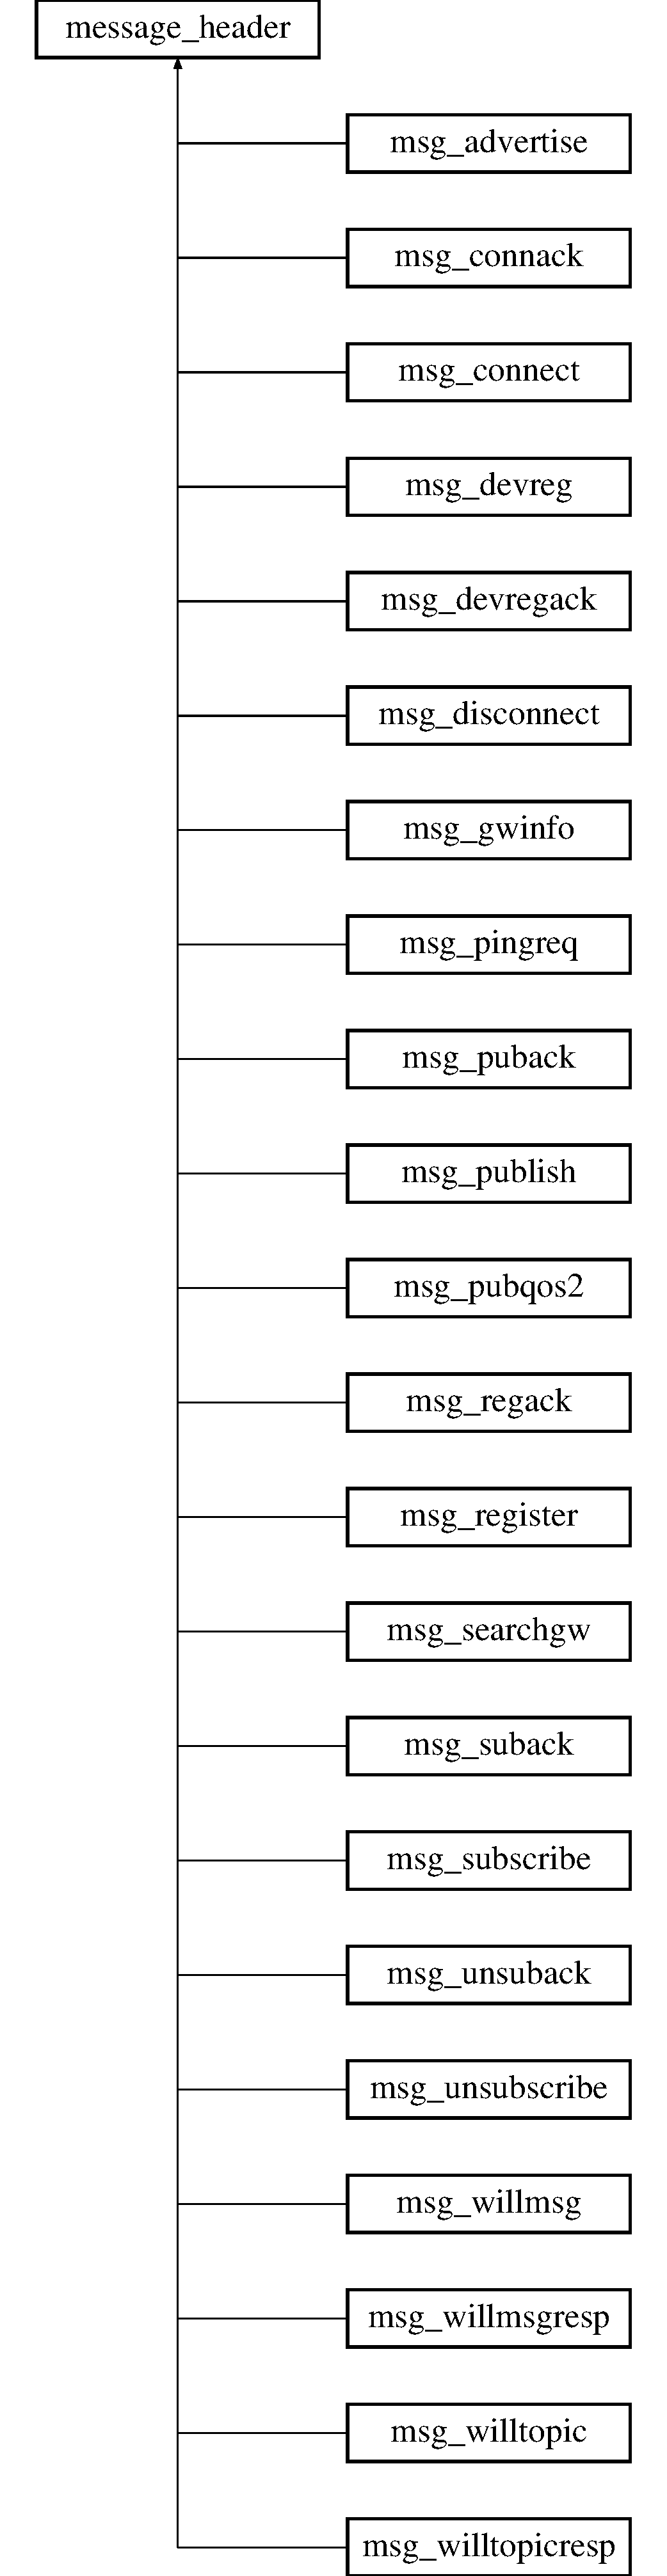
\includegraphics[height=12.000000cm]{structmessage__header}
\end{center}
\end{figure}
\subsection*{Public Attributes}
\begin{DoxyCompactItemize}
\item 
\hypertarget{structmessage__header_a8b6faf1d2a226e583d76d197cde1fff0}{uint8\-\_\-t {\bfseries length}}\label{structmessage__header_a8b6faf1d2a226e583d76d197cde1fff0}

\item 
\hypertarget{structmessage__header_ac23a31e93b17daaff54136321916b583}{uint8\-\_\-t {\bfseries type}}\label{structmessage__header_ac23a31e93b17daaff54136321916b583}

\end{DoxyCompactItemize}


The documentation for this struct was generated from the following file\-:\begin{DoxyCompactItemize}
\item 
\hyperlink{thing__defines_8h}{thing\-\_\-defines.\-h}\end{DoxyCompactItemize}

\hypertarget{structmsg__advertise}{\section{msg\-\_\-advertise Struct Reference}
\label{structmsg__advertise}\index{msg\-\_\-advertise@{msg\-\_\-advertise}}
}
Inheritance diagram for msg\-\_\-advertise\-:\begin{figure}[H]
\begin{center}
\leavevmode
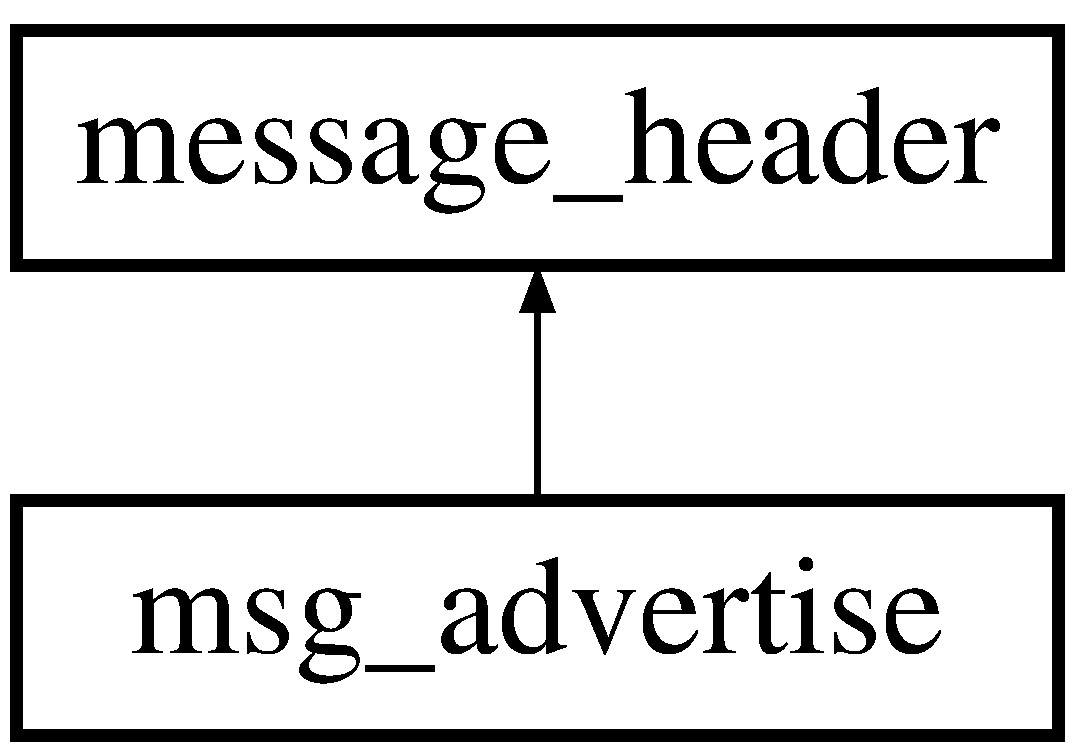
\includegraphics[height=2.000000cm]{structmsg__advertise}
\end{center}
\end{figure}
\subsection*{Public Attributes}
\begin{DoxyCompactItemize}
\item 
\hypertarget{structmsg__advertise_a7bc4dcaae7dbd6d72f2a262259ee83c6}{uint8\-\_\-t {\bfseries gw\-\_\-id}}\label{structmsg__advertise_a7bc4dcaae7dbd6d72f2a262259ee83c6}

\item 
\hypertarget{structmsg__advertise_ae3abc7389105209dfec94092ff837128}{uint16\-\_\-t {\bfseries duration}}\label{structmsg__advertise_ae3abc7389105209dfec94092ff837128}

\end{DoxyCompactItemize}


The documentation for this struct was generated from the following file\-:\begin{DoxyCompactItemize}
\item 
\hyperlink{thing__defines_8h}{thing\-\_\-defines.\-h}\end{DoxyCompactItemize}

\hypertarget{structmsg__connack}{\section{msg\-\_\-connack Struct Reference}
\label{structmsg__connack}\index{msg\-\_\-connack@{msg\-\_\-connack}}
}
Inheritance diagram for msg\-\_\-connack\-:\begin{figure}[H]
\begin{center}
\leavevmode
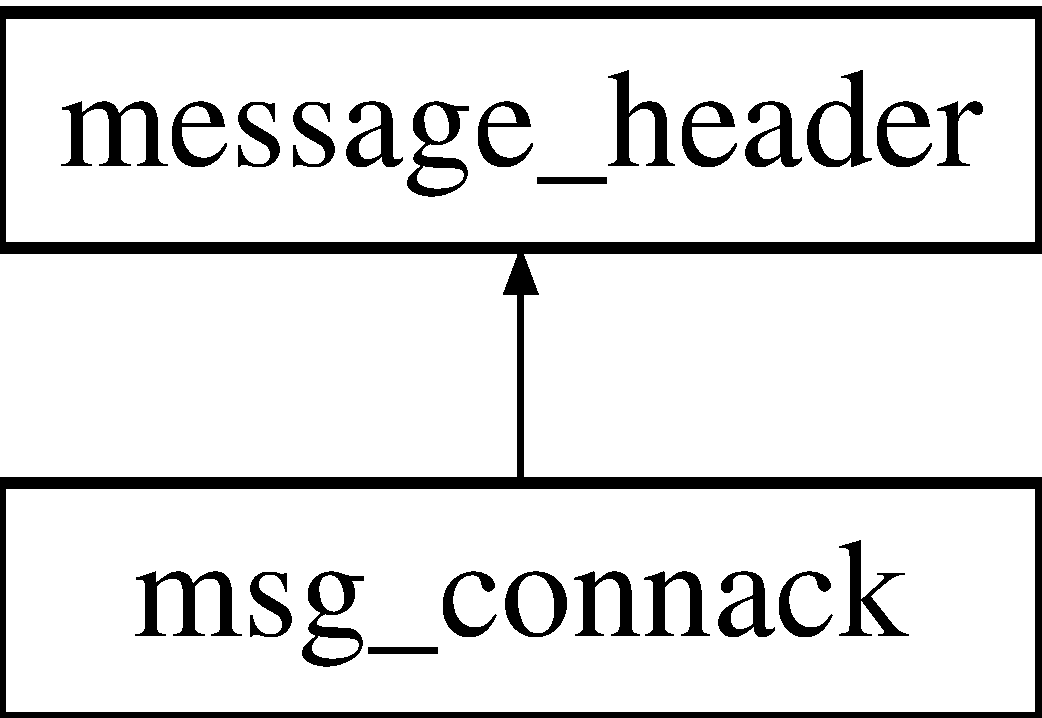
\includegraphics[height=2.000000cm]{structmsg__connack}
\end{center}
\end{figure}
\subsection*{Public Attributes}
\begin{DoxyCompactItemize}
\item 
\hypertarget{structmsg__connack_ac8771823991ca3e61b7c44d63dd4a124}{return\-\_\-code\-\_\-t {\bfseries return\-\_\-code}}\label{structmsg__connack_ac8771823991ca3e61b7c44d63dd4a124}

\end{DoxyCompactItemize}


The documentation for this struct was generated from the following file\-:\begin{DoxyCompactItemize}
\item 
\hyperlink{thing__defines_8h}{thing\-\_\-defines.\-h}\end{DoxyCompactItemize}

\hypertarget{structmsg__connect}{\section{msg\-\_\-connect Struct Reference}
\label{structmsg__connect}\index{msg\-\_\-connect@{msg\-\_\-connect}}
}
Inheritance diagram for msg\-\_\-connect\-:\begin{figure}[H]
\begin{center}
\leavevmode
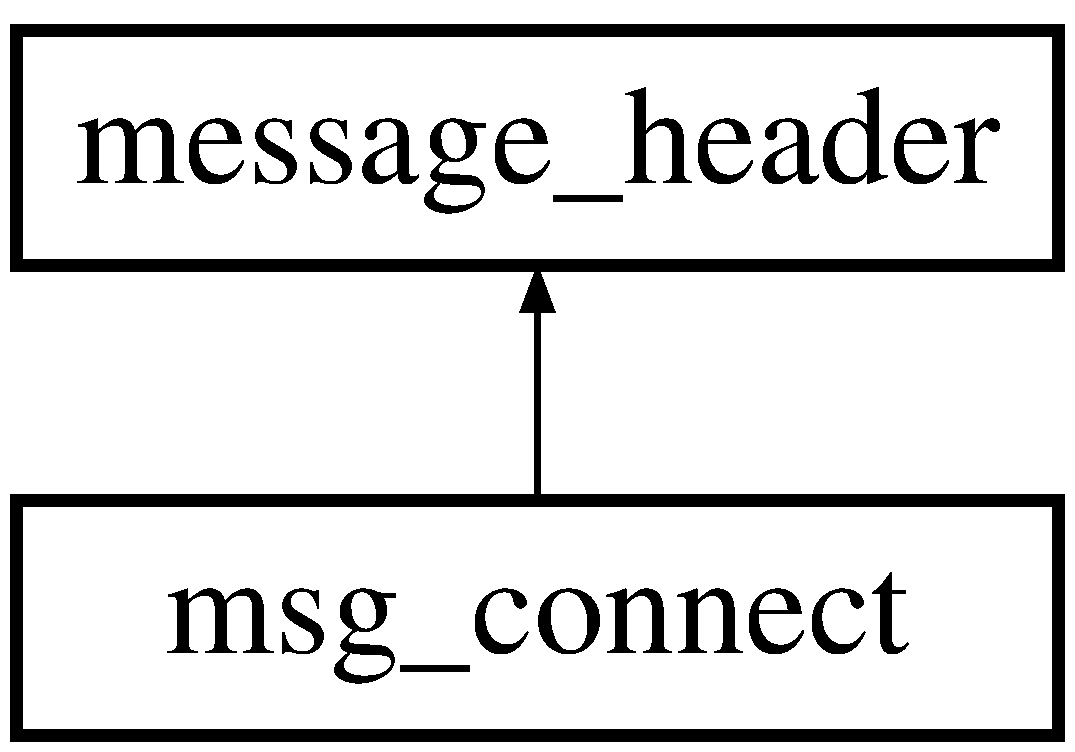
\includegraphics[height=2.000000cm]{structmsg__connect}
\end{center}
\end{figure}
\subsection*{Public Attributes}
\begin{DoxyCompactItemize}
\item 
\hypertarget{structmsg__connect_a4fc0429270b074f1d074ba54bc4865dc}{uint8\-\_\-t {\bfseries flags}}\label{structmsg__connect_a4fc0429270b074f1d074ba54bc4865dc}

\item 
\hypertarget{structmsg__connect_a44a19851855343532dbbd64f35c96fae}{uint8\-\_\-t {\bfseries protocol\-\_\-id}}\label{structmsg__connect_a44a19851855343532dbbd64f35c96fae}

\item 
\hypertarget{structmsg__connect_a2b0f638095ccc0d4c408118c4a2cb0a2}{uint16\-\_\-t {\bfseries duration}}\label{structmsg__connect_a2b0f638095ccc0d4c408118c4a2cb0a2}

\item 
\hypertarget{structmsg__connect_a11a6095b393802c198d3e14e19f630ae}{char {\bfseries client\-\_\-id} \mbox{[}0\mbox{]}}\label{structmsg__connect_a11a6095b393802c198d3e14e19f630ae}

\end{DoxyCompactItemize}


The documentation for this struct was generated from the following file\-:\begin{DoxyCompactItemize}
\item 
\hyperlink{thing__defines_8h}{thing\-\_\-defines.\-h}\end{DoxyCompactItemize}

\hypertarget{structmsg__devreg}{\section{msg\-\_\-devreg Struct Reference}
\label{structmsg__devreg}\index{msg\-\_\-devreg@{msg\-\_\-devreg}}
}
Inheritance diagram for msg\-\_\-devreg\-:\begin{figure}[H]
\begin{center}
\leavevmode
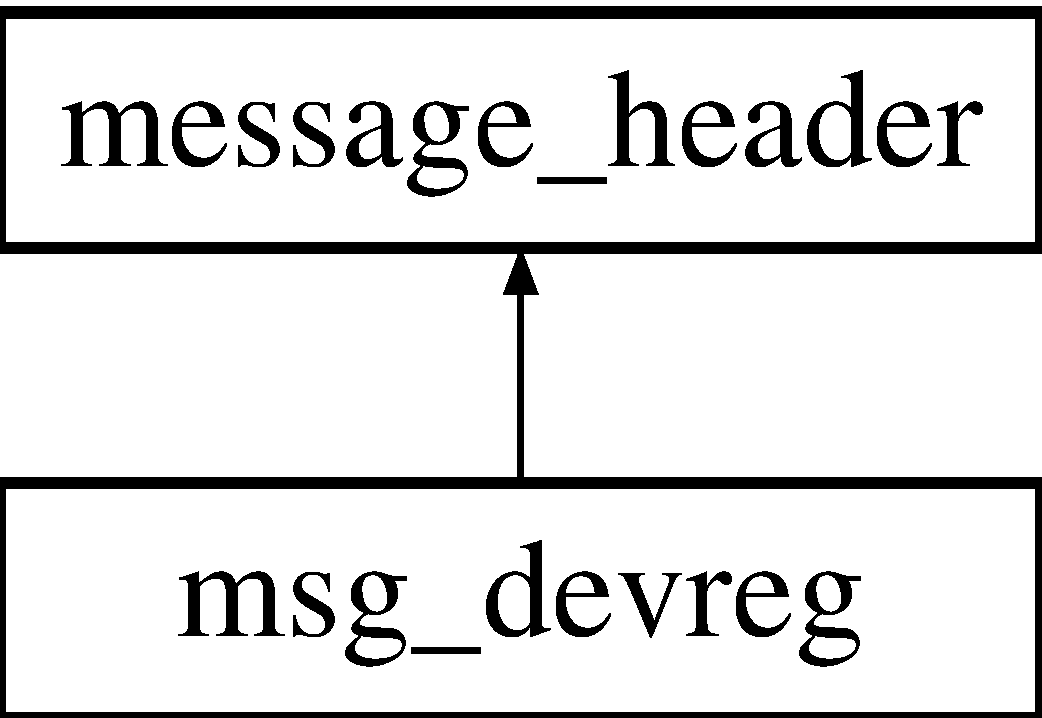
\includegraphics[height=2.000000cm]{structmsg__devreg}
\end{center}
\end{figure}
\subsection*{Public Attributes}
\begin{DoxyCompactItemize}
\item 
\hypertarget{structmsg__devreg_a77888724fda6f1adac16d4a346bd84be}{uint16\-\_\-t {\bfseries pub\-\_\-id}}\label{structmsg__devreg_a77888724fda6f1adac16d4a346bd84be}

\item 
\hypertarget{structmsg__devreg_a4da49bb64f4800ae14644439974108fc}{uint16\-\_\-t {\bfseries message\-\_\-id}}\label{structmsg__devreg_a4da49bb64f4800ae14644439974108fc}

\item 
\hypertarget{structmsg__devreg_ab669c3e7543979798cc5bf9b9cc1ea47}{uint8\-\_\-t {\bfseries status}}\label{structmsg__devreg_ab669c3e7543979798cc5bf9b9cc1ea47}

\item 
\hypertarget{structmsg__devreg_af0494e12edecd91bf4add32d2fe610c0}{char {\bfseries data} \mbox{[}0\mbox{]}}\label{structmsg__devreg_af0494e12edecd91bf4add32d2fe610c0}

\end{DoxyCompactItemize}


The documentation for this struct was generated from the following file\-:\begin{DoxyCompactItemize}
\item 
\hyperlink{thing__defines_8h}{thing\-\_\-defines.\-h}\end{DoxyCompactItemize}

\hypertarget{structmsg__devregack}{\section{msg\-\_\-devregack Struct Reference}
\label{structmsg__devregack}\index{msg\-\_\-devregack@{msg\-\_\-devregack}}
}
Inheritance diagram for msg\-\_\-devregack\-:\begin{figure}[H]
\begin{center}
\leavevmode
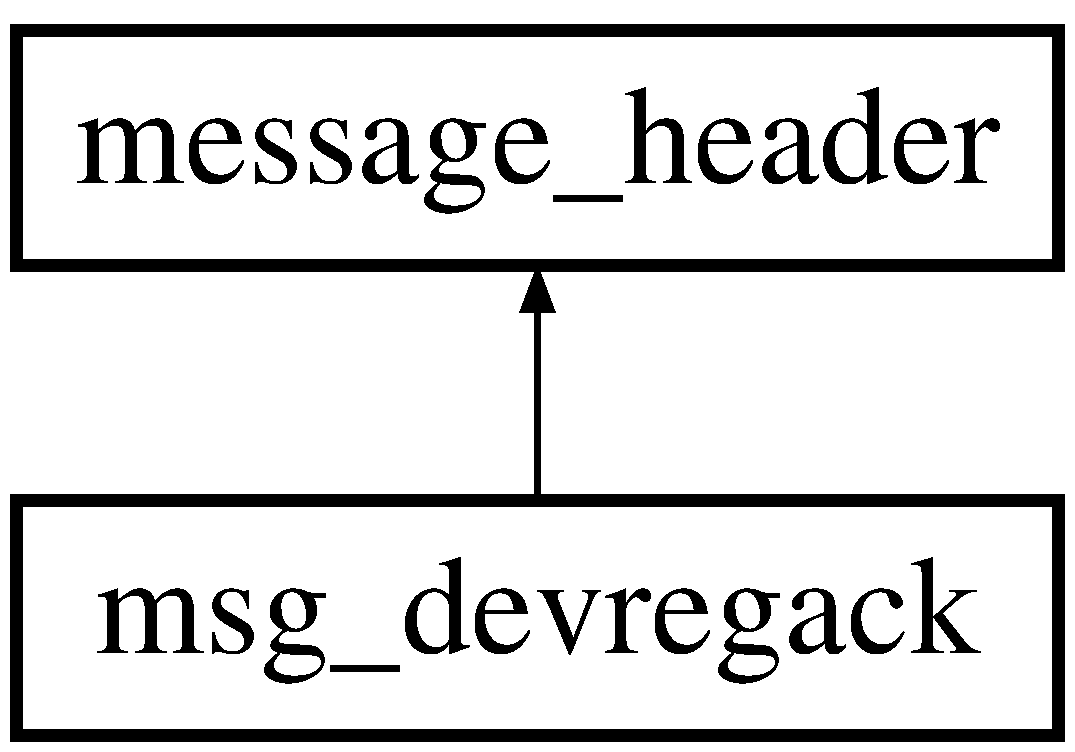
\includegraphics[height=2.000000cm]{structmsg__devregack}
\end{center}
\end{figure}
\subsection*{Public Attributes}
\begin{DoxyCompactItemize}
\item 
\hypertarget{structmsg__devregack_a4ef800c8c034925f97df8aea1df64ff6}{uint8\-\_\-t {\bfseries flags}}\label{structmsg__devregack_a4ef800c8c034925f97df8aea1df64ff6}

\item 
\hypertarget{structmsg__devregack_ab8a8e50decda829198f79e5100df30c2}{uint16\-\_\-t {\bfseries message\-\_\-id}}\label{structmsg__devregack_ab8a8e50decda829198f79e5100df30c2}

\item 
\hypertarget{structmsg__devregack_ab339916c12670ceb2845cfded76c87fd}{uint8\-\_\-t {\bfseries return\-\_\-code}}\label{structmsg__devregack_ab339916c12670ceb2845cfded76c87fd}

\end{DoxyCompactItemize}


The documentation for this struct was generated from the following file\-:\begin{DoxyCompactItemize}
\item 
\hyperlink{thing__defines_8h}{thing\-\_\-defines.\-h}\end{DoxyCompactItemize}

\hypertarget{structmsg__disconnect}{\section{msg\-\_\-disconnect Struct Reference}
\label{structmsg__disconnect}\index{msg\-\_\-disconnect@{msg\-\_\-disconnect}}
}
Inheritance diagram for msg\-\_\-disconnect\-:\begin{figure}[H]
\begin{center}
\leavevmode
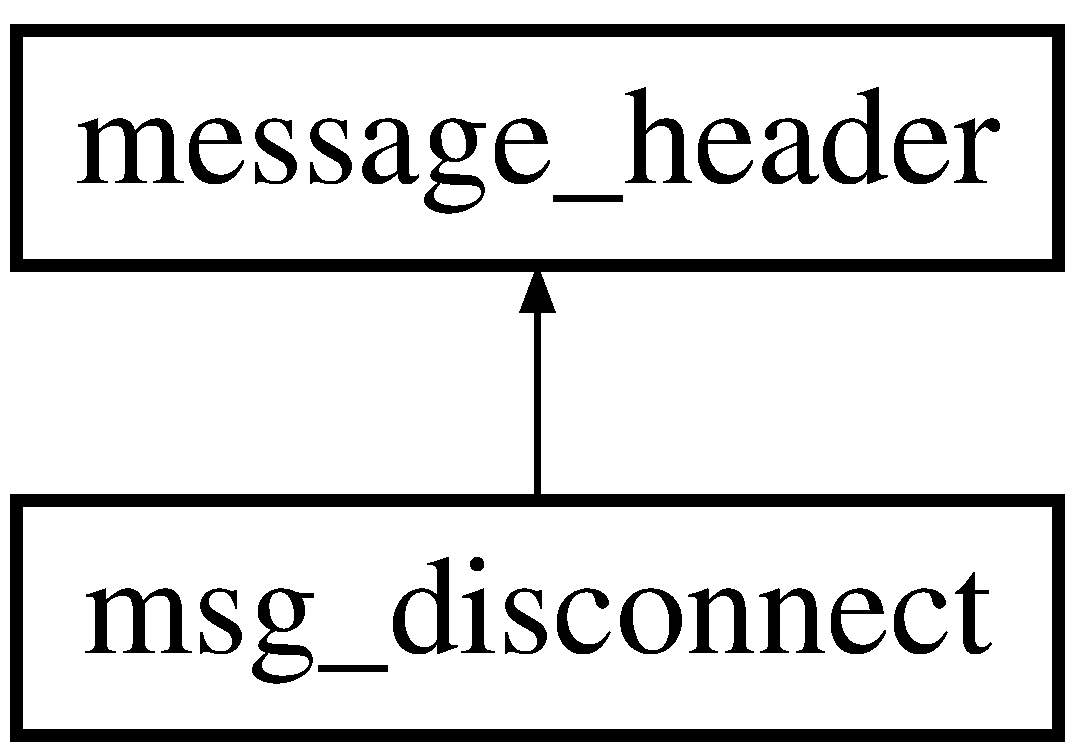
\includegraphics[height=2.000000cm]{structmsg__disconnect}
\end{center}
\end{figure}
\subsection*{Public Attributes}
\begin{DoxyCompactItemize}
\item 
\hypertarget{structmsg__disconnect_a242651c3b5beda3022d26cd6bf12dc49}{uint16\-\_\-t {\bfseries duration}}\label{structmsg__disconnect_a242651c3b5beda3022d26cd6bf12dc49}

\end{DoxyCompactItemize}


The documentation for this struct was generated from the following file\-:\begin{DoxyCompactItemize}
\item 
\hyperlink{thing__defines_8h}{thing\-\_\-defines.\-h}\end{DoxyCompactItemize}

\hypertarget{structmsg__gwinfo}{\section{msg\-\_\-gwinfo Struct Reference}
\label{structmsg__gwinfo}\index{msg\-\_\-gwinfo@{msg\-\_\-gwinfo}}
}
Inheritance diagram for msg\-\_\-gwinfo\-:\begin{figure}[H]
\begin{center}
\leavevmode
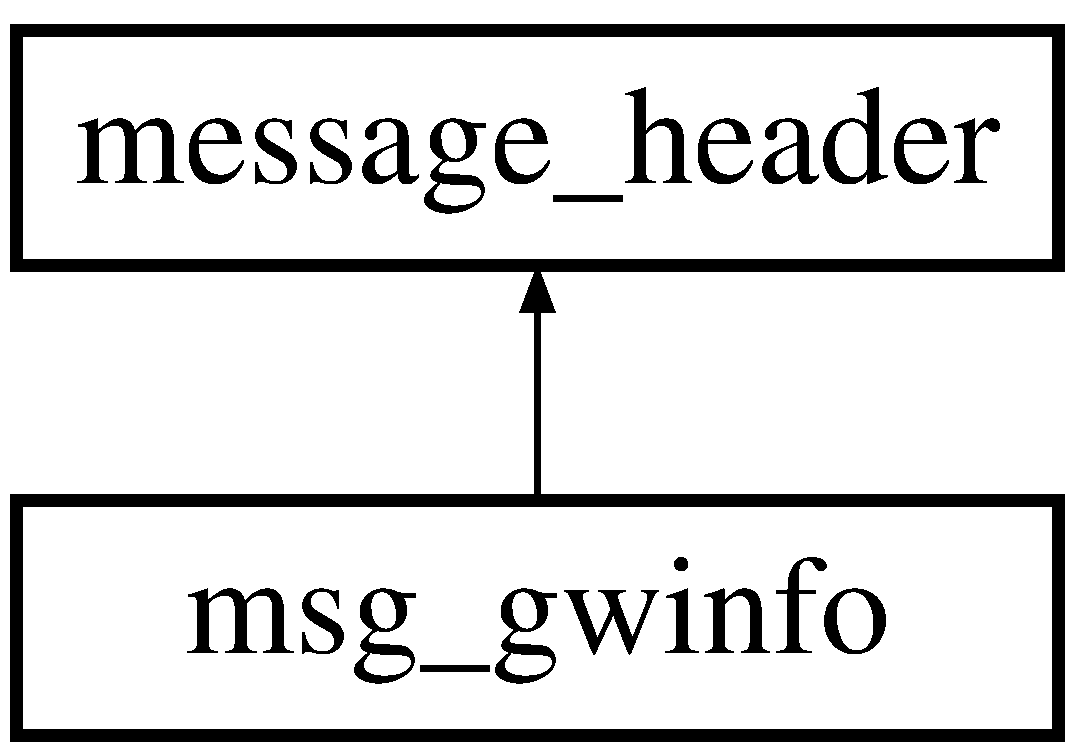
\includegraphics[height=2.000000cm]{structmsg__gwinfo}
\end{center}
\end{figure}
\subsection*{Public Attributes}
\begin{DoxyCompactItemize}
\item 
\hypertarget{structmsg__gwinfo_a726983d8610681306248b0a6d49b09f0}{uint8\-\_\-t {\bfseries gw\-\_\-id}}\label{structmsg__gwinfo_a726983d8610681306248b0a6d49b09f0}

\item 
\hypertarget{structmsg__gwinfo_a7895025f94b89f5f0737caa659313b86}{char {\bfseries gw\-\_\-add} \mbox{[}0\mbox{]}}\label{structmsg__gwinfo_a7895025f94b89f5f0737caa659313b86}

\end{DoxyCompactItemize}


The documentation for this struct was generated from the following file\-:\begin{DoxyCompactItemize}
\item 
\hyperlink{thing__defines_8h}{thing\-\_\-defines.\-h}\end{DoxyCompactItemize}

\hypertarget{structmsg__pingreq}{\section{msg\-\_\-pingreq Struct Reference}
\label{structmsg__pingreq}\index{msg\-\_\-pingreq@{msg\-\_\-pingreq}}
}
Inheritance diagram for msg\-\_\-pingreq\-:\begin{figure}[H]
\begin{center}
\leavevmode
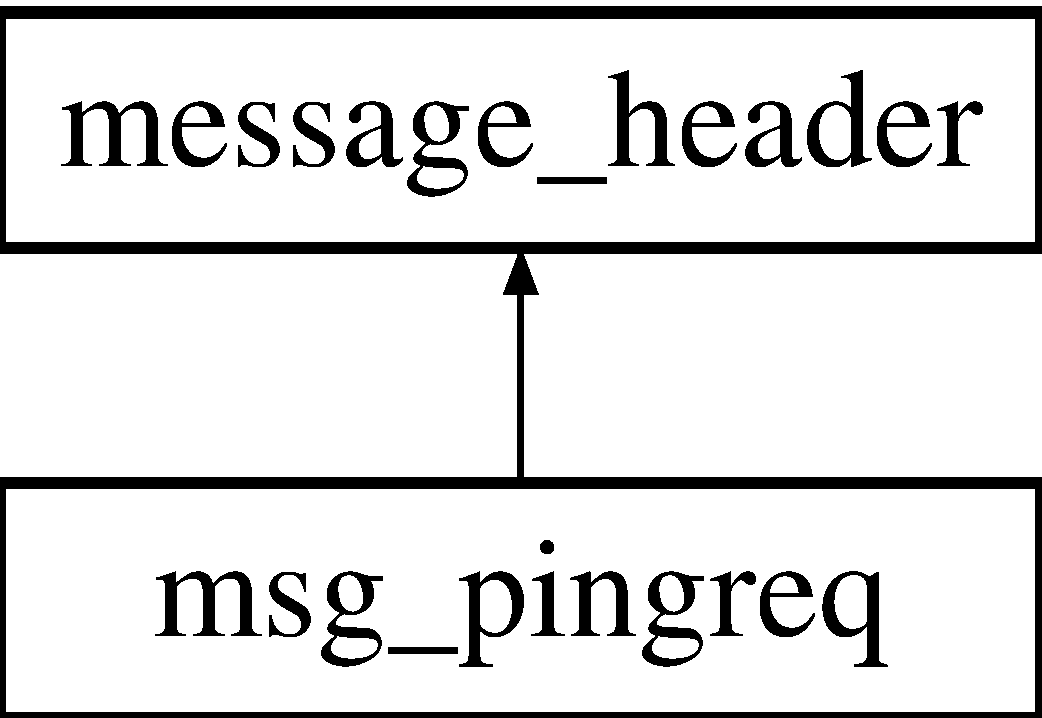
\includegraphics[height=2.000000cm]{structmsg__pingreq}
\end{center}
\end{figure}
\subsection*{Public Attributes}
\begin{DoxyCompactItemize}
\item 
\hypertarget{structmsg__pingreq_a0c9e844a39e481ebf6e061bbca5f326f}{char {\bfseries client\-\_\-id} \mbox{[}0\mbox{]}}\label{structmsg__pingreq_a0c9e844a39e481ebf6e061bbca5f326f}

\end{DoxyCompactItemize}


The documentation for this struct was generated from the following file\-:\begin{DoxyCompactItemize}
\item 
\hyperlink{thing__defines_8h}{thing\-\_\-defines.\-h}\end{DoxyCompactItemize}

\hypertarget{structmsg__puback}{\section{msg\-\_\-puback Struct Reference}
\label{structmsg__puback}\index{msg\-\_\-puback@{msg\-\_\-puback}}
}
Inheritance diagram for msg\-\_\-puback\-:\begin{figure}[H]
\begin{center}
\leavevmode
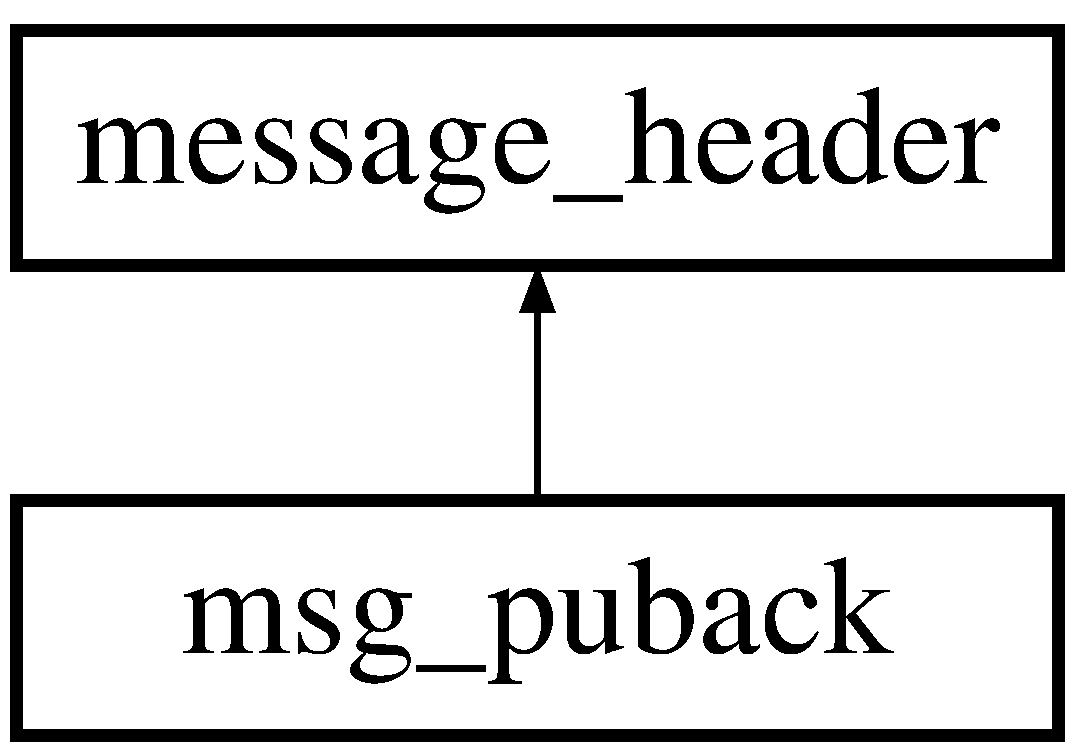
\includegraphics[height=2.000000cm]{structmsg__puback}
\end{center}
\end{figure}
\subsection*{Public Attributes}
\begin{DoxyCompactItemize}
\item 
\hypertarget{structmsg__puback_aaee5d68fe5a9286fe293f0081f2c446c}{uint16\-\_\-t {\bfseries topic\-\_\-id}}\label{structmsg__puback_aaee5d68fe5a9286fe293f0081f2c446c}

\item 
\hypertarget{structmsg__puback_a8524df10b62eaa70ad043971fba54370}{uint16\-\_\-t {\bfseries message\-\_\-id}}\label{structmsg__puback_a8524df10b62eaa70ad043971fba54370}

\item 
\hypertarget{structmsg__puback_a3645248497ed231a2404b78df4798d6d}{uint8\-\_\-t {\bfseries return\-\_\-code}}\label{structmsg__puback_a3645248497ed231a2404b78df4798d6d}

\end{DoxyCompactItemize}


The documentation for this struct was generated from the following file\-:\begin{DoxyCompactItemize}
\item 
\hyperlink{thing__defines_8h}{thing\-\_\-defines.\-h}\end{DoxyCompactItemize}

\hypertarget{structmsg__publish}{\section{msg\-\_\-publish Struct Reference}
\label{structmsg__publish}\index{msg\-\_\-publish@{msg\-\_\-publish}}
}
Inheritance diagram for msg\-\_\-publish\-:\begin{figure}[H]
\begin{center}
\leavevmode
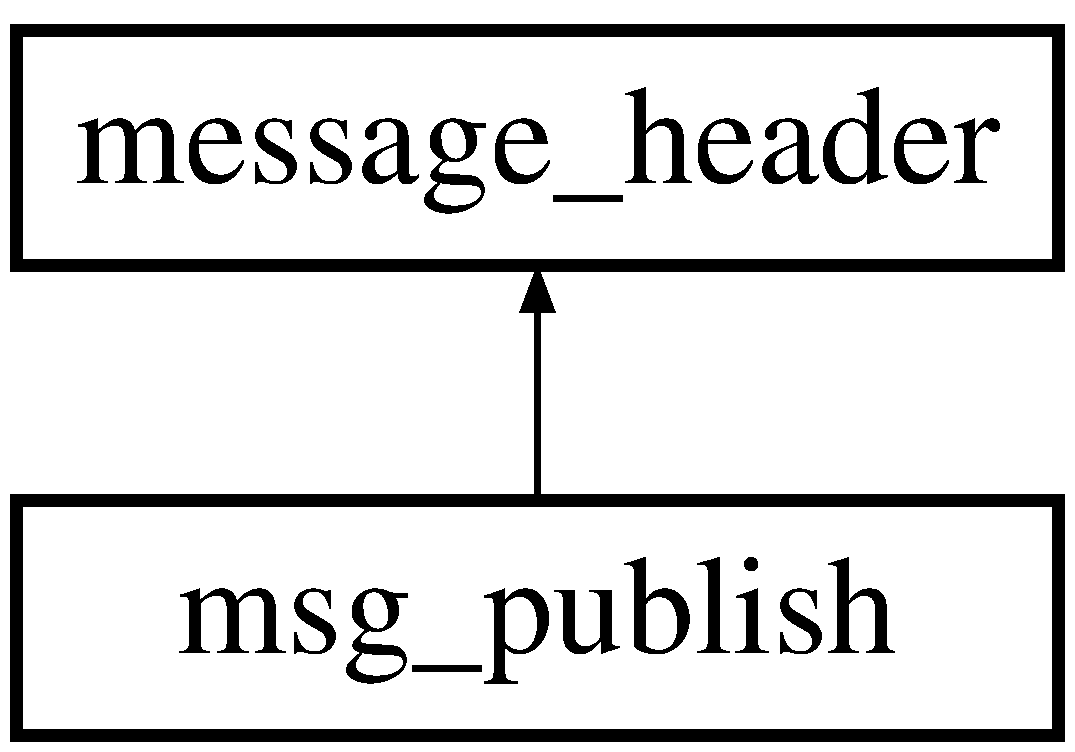
\includegraphics[height=2.000000cm]{structmsg__publish}
\end{center}
\end{figure}
\subsection*{Public Attributes}
\begin{DoxyCompactItemize}
\item 
\hypertarget{structmsg__publish_ad88a1705431981521d2d75e7ce6d42f9}{uint8\-\_\-t {\bfseries flags}}\label{structmsg__publish_ad88a1705431981521d2d75e7ce6d42f9}

\item 
\hypertarget{structmsg__publish_a3773e07cdce2514dd471d6a7aae9ea0d}{uint16\-\_\-t {\bfseries topic\-\_\-id}}\label{structmsg__publish_a3773e07cdce2514dd471d6a7aae9ea0d}

\item 
\hypertarget{structmsg__publish_a736e8364ba9d40e4ead603870064cdfd}{uint16\-\_\-t {\bfseries message\-\_\-id}}\label{structmsg__publish_a736e8364ba9d40e4ead603870064cdfd}

\item 
\hypertarget{structmsg__publish_a24874a8acba3dc087ff98d915031cf16}{char {\bfseries data} \mbox{[}0\mbox{]}}\label{structmsg__publish_a24874a8acba3dc087ff98d915031cf16}

\end{DoxyCompactItemize}


The documentation for this struct was generated from the following file\-:\begin{DoxyCompactItemize}
\item 
\hyperlink{thing__defines_8h}{thing\-\_\-defines.\-h}\end{DoxyCompactItemize}

\hypertarget{structmsg__pubqos2}{\section{msg\-\_\-pubqos2 Struct Reference}
\label{structmsg__pubqos2}\index{msg\-\_\-pubqos2@{msg\-\_\-pubqos2}}
}
Inheritance diagram for msg\-\_\-pubqos2\-:\begin{figure}[H]
\begin{center}
\leavevmode
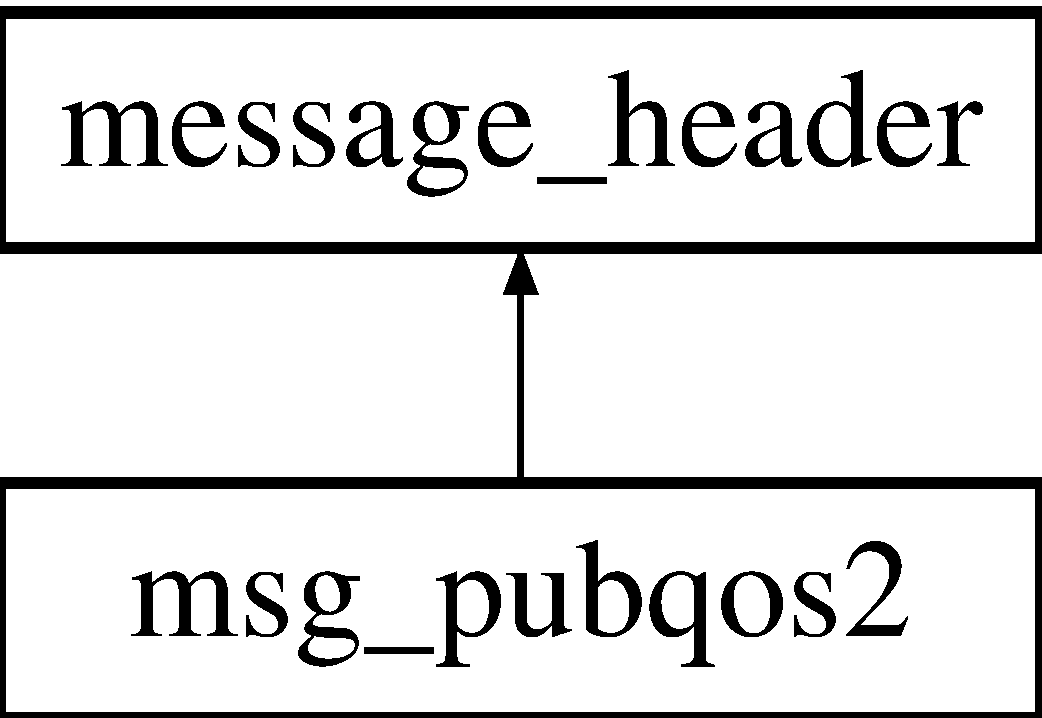
\includegraphics[height=2.000000cm]{structmsg__pubqos2}
\end{center}
\end{figure}
\subsection*{Public Attributes}
\begin{DoxyCompactItemize}
\item 
\hypertarget{structmsg__pubqos2_ae17a54c533fc396b23e990bae6feb48f}{uint16\-\_\-t {\bfseries message\-\_\-id}}\label{structmsg__pubqos2_ae17a54c533fc396b23e990bae6feb48f}

\end{DoxyCompactItemize}


The documentation for this struct was generated from the following file\-:\begin{DoxyCompactItemize}
\item 
\hyperlink{thing__defines_8h}{thing\-\_\-defines.\-h}\end{DoxyCompactItemize}

\hypertarget{structmsg__regack}{\section{msg\-\_\-regack Struct Reference}
\label{structmsg__regack}\index{msg\-\_\-regack@{msg\-\_\-regack}}
}
Inheritance diagram for msg\-\_\-regack\-:\begin{figure}[H]
\begin{center}
\leavevmode
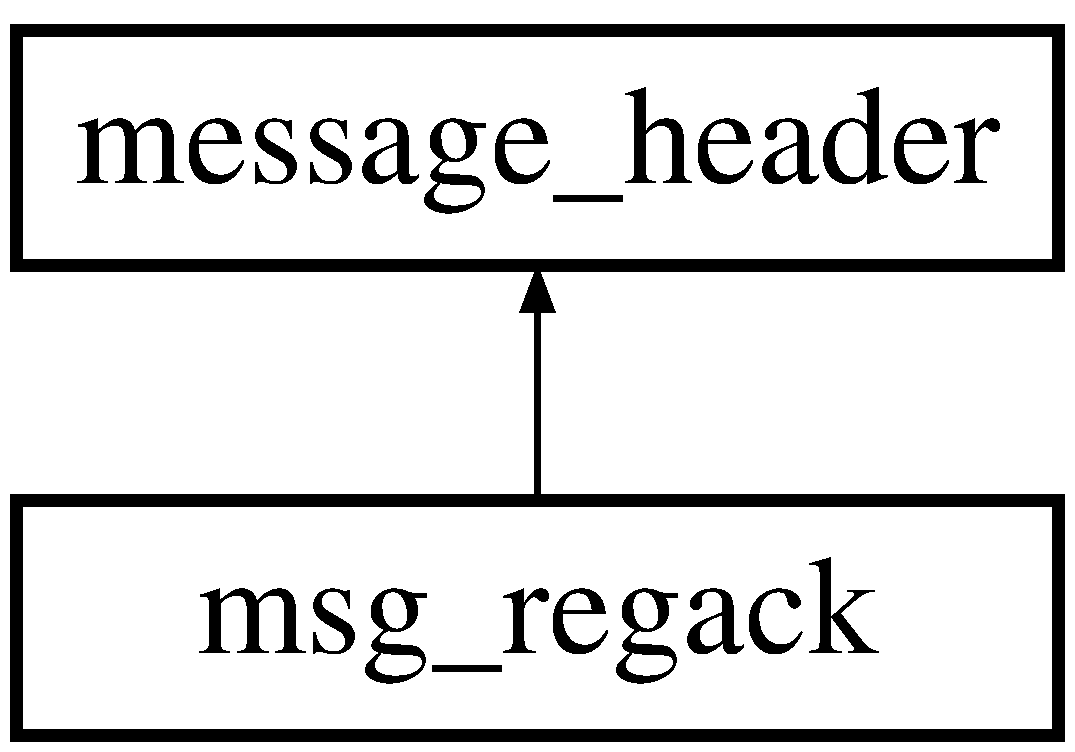
\includegraphics[height=2.000000cm]{structmsg__regack}
\end{center}
\end{figure}
\subsection*{Public Attributes}
\begin{DoxyCompactItemize}
\item 
\hypertarget{structmsg__regack_ad3226ef797365afe79888574d4582f8f}{uint16\-\_\-t {\bfseries topic\-\_\-id}}\label{structmsg__regack_ad3226ef797365afe79888574d4582f8f}

\item 
\hypertarget{structmsg__regack_ac036777c051eeeac62927abb797c3a26}{uint16\-\_\-t {\bfseries message\-\_\-id}}\label{structmsg__regack_ac036777c051eeeac62927abb797c3a26}

\item 
\hypertarget{structmsg__regack_a7b3a7992c75e123416d68648bc59892e}{uint8\-\_\-t {\bfseries return\-\_\-code}}\label{structmsg__regack_a7b3a7992c75e123416d68648bc59892e}

\end{DoxyCompactItemize}


The documentation for this struct was generated from the following file\-:\begin{DoxyCompactItemize}
\item 
\hyperlink{thing__defines_8h}{thing\-\_\-defines.\-h}\end{DoxyCompactItemize}

\hypertarget{structmsg__register}{\section{msg\-\_\-register Struct Reference}
\label{structmsg__register}\index{msg\-\_\-register@{msg\-\_\-register}}
}
Inheritance diagram for msg\-\_\-register\-:\begin{figure}[H]
\begin{center}
\leavevmode
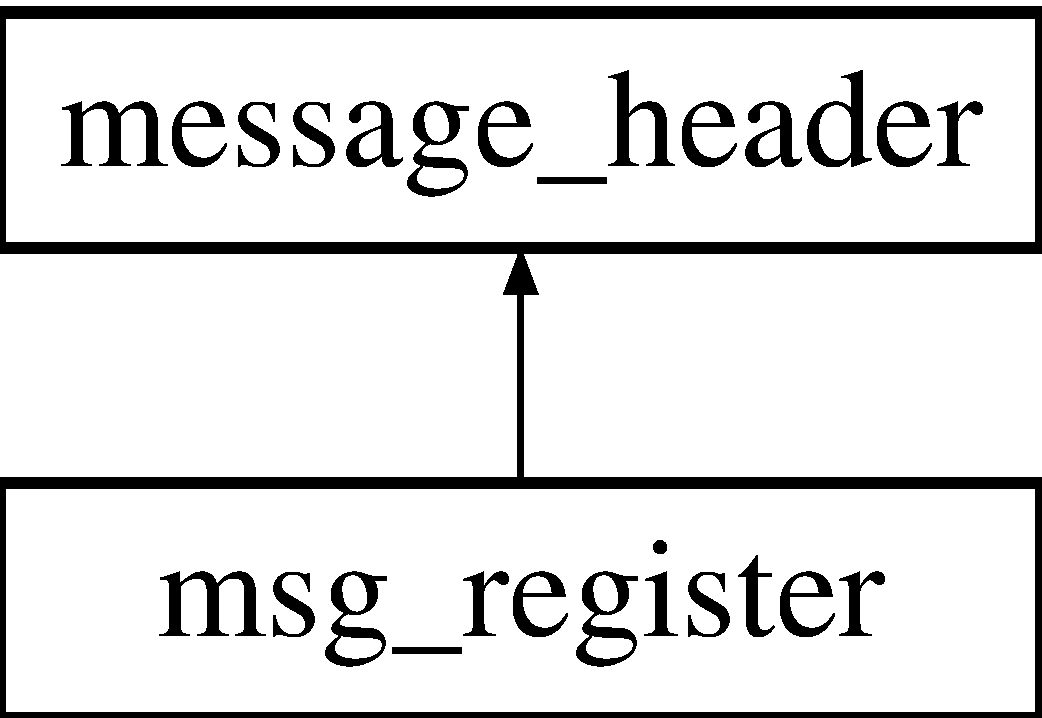
\includegraphics[height=2.000000cm]{structmsg__register}
\end{center}
\end{figure}
\subsection*{Public Attributes}
\begin{DoxyCompactItemize}
\item 
\hypertarget{structmsg__register_ad99373ef209dd1bc1ac76cf00b38483a}{uint16\-\_\-t {\bfseries topic\-\_\-id}}\label{structmsg__register_ad99373ef209dd1bc1ac76cf00b38483a}

\item 
\hypertarget{structmsg__register_a069b62ae801b9a413b293b0939b2b685}{uint16\-\_\-t {\bfseries message\-\_\-id}}\label{structmsg__register_a069b62ae801b9a413b293b0939b2b685}

\item 
\hypertarget{structmsg__register_ae2399455c0b7f86010781bf6e37ab619}{char {\bfseries topic\-\_\-name} \mbox{[}0\mbox{]}}\label{structmsg__register_ae2399455c0b7f86010781bf6e37ab619}

\end{DoxyCompactItemize}


The documentation for this struct was generated from the following file\-:\begin{DoxyCompactItemize}
\item 
\hyperlink{thing__defines_8h}{thing\-\_\-defines.\-h}\end{DoxyCompactItemize}

\hypertarget{structmsg__searchgw}{\section{msg\-\_\-searchgw Struct Reference}
\label{structmsg__searchgw}\index{msg\-\_\-searchgw@{msg\-\_\-searchgw}}
}
Inheritance diagram for msg\-\_\-searchgw\-:\begin{figure}[H]
\begin{center}
\leavevmode
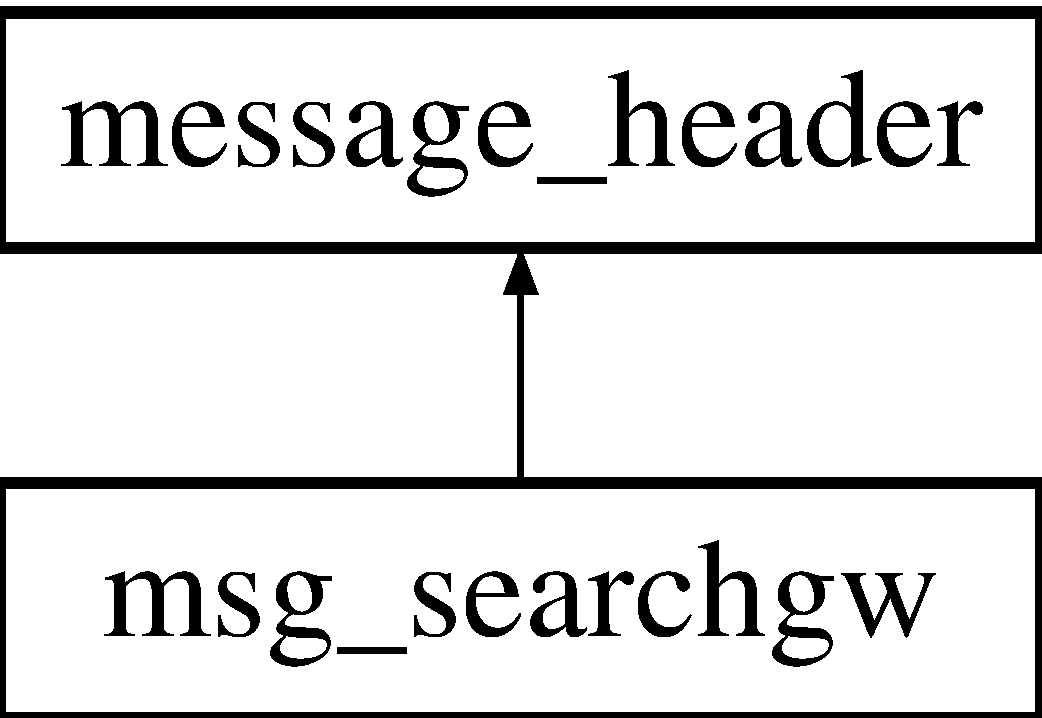
\includegraphics[height=2.000000cm]{structmsg__searchgw}
\end{center}
\end{figure}
\subsection*{Public Attributes}
\begin{DoxyCompactItemize}
\item 
\hypertarget{structmsg__searchgw_aeb357d8594fb3d9f0e9f694a01776179}{uint8\-\_\-t {\bfseries radius}}\label{structmsg__searchgw_aeb357d8594fb3d9f0e9f694a01776179}

\end{DoxyCompactItemize}


The documentation for this struct was generated from the following file\-:\begin{DoxyCompactItemize}
\item 
\hyperlink{thing__defines_8h}{thing\-\_\-defines.\-h}\end{DoxyCompactItemize}

\hypertarget{structmsg__suback}{\section{msg\-\_\-suback Struct Reference}
\label{structmsg__suback}\index{msg\-\_\-suback@{msg\-\_\-suback}}
}
Inheritance diagram for msg\-\_\-suback\-:\begin{figure}[H]
\begin{center}
\leavevmode
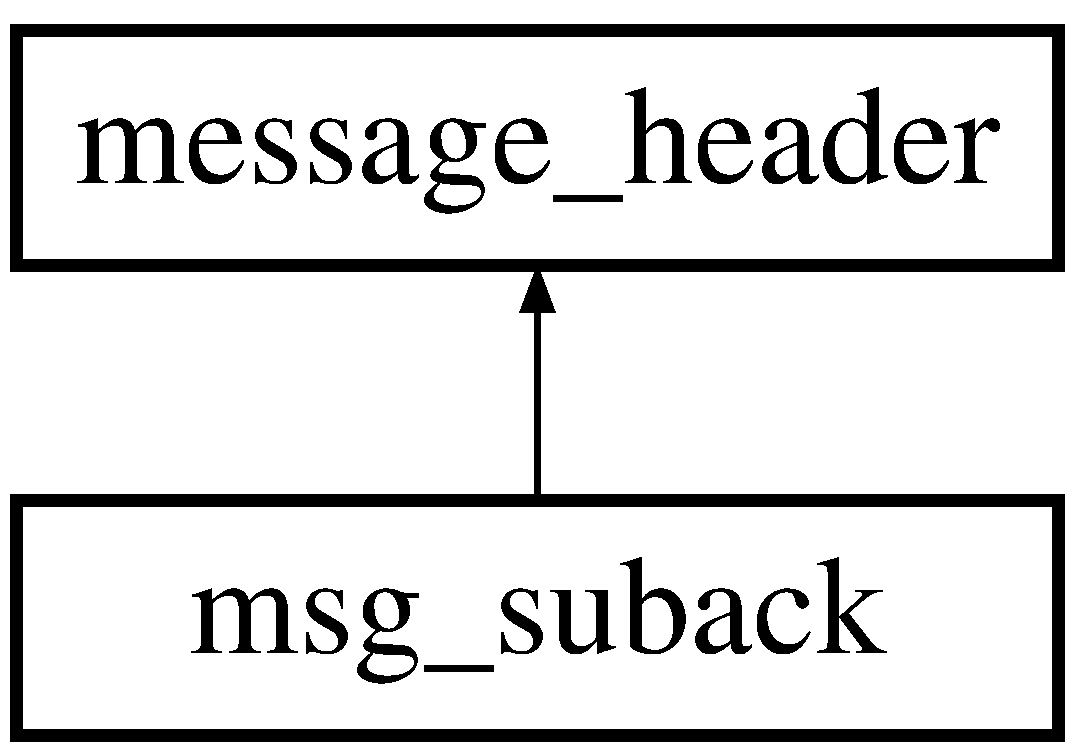
\includegraphics[height=2.000000cm]{structmsg__suback}
\end{center}
\end{figure}
\subsection*{Public Attributes}
\begin{DoxyCompactItemize}
\item 
\hypertarget{structmsg__suback_ad36871bff8bdd84269560fef37072764}{uint8\-\_\-t {\bfseries flags}}\label{structmsg__suback_ad36871bff8bdd84269560fef37072764}

\item 
\hypertarget{structmsg__suback_ac9a614ff568ce6e7ef7cd59d8700f7ca}{uint16\-\_\-t {\bfseries topic\-\_\-id}}\label{structmsg__suback_ac9a614ff568ce6e7ef7cd59d8700f7ca}

\item 
\hypertarget{structmsg__suback_ad8420b6b42af00251b95518bf42771dd}{uint16\-\_\-t {\bfseries message\-\_\-id}}\label{structmsg__suback_ad8420b6b42af00251b95518bf42771dd}

\item 
\hypertarget{structmsg__suback_a8896e294abd8a05e37151965fed1e794}{uint8\-\_\-t {\bfseries return\-\_\-code}}\label{structmsg__suback_a8896e294abd8a05e37151965fed1e794}

\end{DoxyCompactItemize}


The documentation for this struct was generated from the following file\-:\begin{DoxyCompactItemize}
\item 
\hyperlink{thing__defines_8h}{thing\-\_\-defines.\-h}\end{DoxyCompactItemize}

\hypertarget{structmsg__subscribe}{\section{msg\-\_\-subscribe Struct Reference}
\label{structmsg__subscribe}\index{msg\-\_\-subscribe@{msg\-\_\-subscribe}}
}
Inheritance diagram for msg\-\_\-subscribe\-:\begin{figure}[H]
\begin{center}
\leavevmode
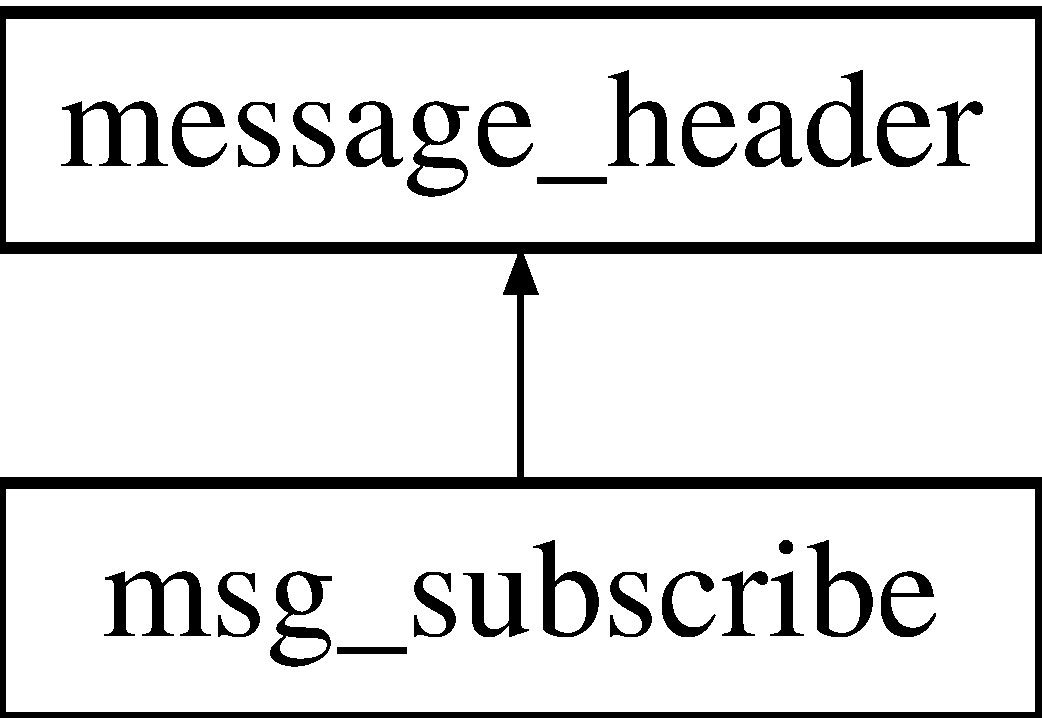
\includegraphics[height=2.000000cm]{structmsg__subscribe}
\end{center}
\end{figure}
\subsection*{Public Attributes}
\begin{DoxyCompactItemize}
\item 
\hypertarget{structmsg__subscribe_a9f5348db4271449d0bcb4baf79ee7996}{uint8\-\_\-t {\bfseries flags}}\label{structmsg__subscribe_a9f5348db4271449d0bcb4baf79ee7996}

\item 
\hypertarget{structmsg__subscribe_a652ab9015af589a606bda6957277d6cb}{uint16\-\_\-t {\bfseries message\-\_\-id}}\label{structmsg__subscribe_a652ab9015af589a606bda6957277d6cb}

\item 
\hypertarget{structmsg__subscribe_afd0442954ce8c755c8c409bef47160c5}{\begin{tabbing}
xx\=xx\=xx\=xx\=xx\=xx\=xx\=xx\=xx\=\kill
union \{\\
\hypertarget{unionmsg__subscribe_1_1@0_a3bbe30e846869f962ddffaefee0cf8f5}{\>char {\bfseries topic\_name} \mbox{[}0\mbox{]}\\
\hypertarget{unionmsg__subscribe_1_1@0_ac3b78169af5cdd3d8686574da7368bd0}{\>uint16\_t {\bfseries topic\_id}\\
\}; }\label{structmsg__subscribe_afd0442954ce8c755c8c409bef47160c5}
\\

\end{tabbing}\end{DoxyCompactItemize}


The documentation for this struct was generated from the following file\-:\begin{DoxyCompactItemize}
\item 
\hyperlink{thing__defines_8h}{thing\-\_\-defines.\-h}\end{DoxyCompactItemize}

\hypertarget{structmsg__unsuback}{\section{msg\-\_\-unsuback Struct Reference}
\label{structmsg__unsuback}\index{msg\-\_\-unsuback@{msg\-\_\-unsuback}}
}
Inheritance diagram for msg\-\_\-unsuback\-:\begin{figure}[H]
\begin{center}
\leavevmode
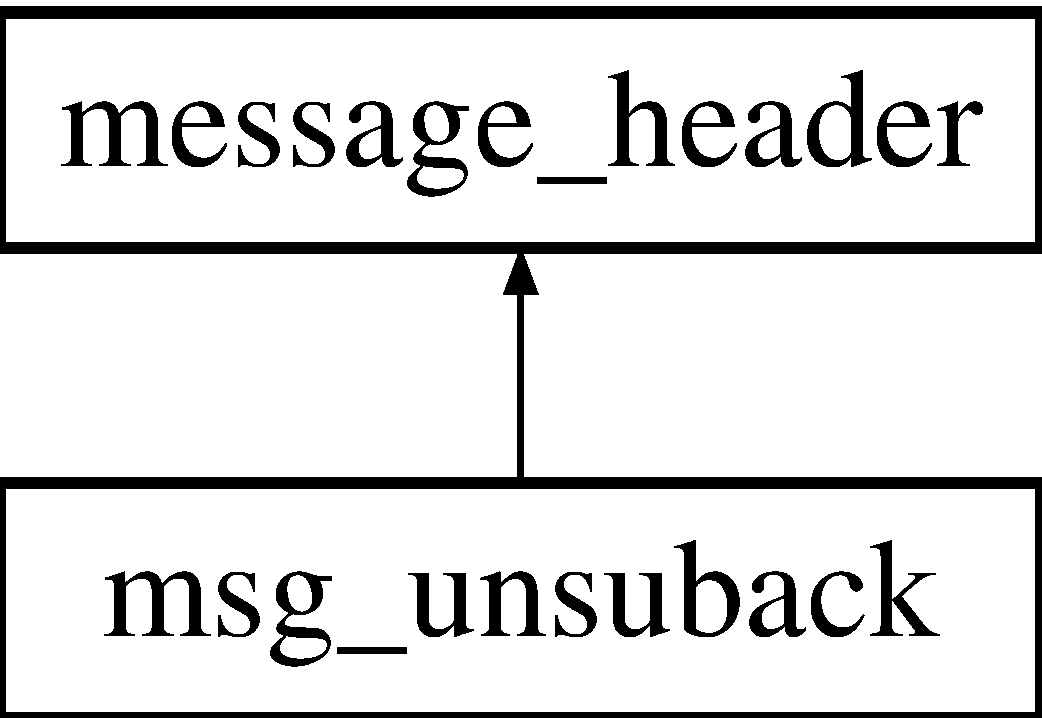
\includegraphics[height=2.000000cm]{structmsg__unsuback}
\end{center}
\end{figure}
\subsection*{Public Attributes}
\begin{DoxyCompactItemize}
\item 
\hypertarget{structmsg__unsuback_aa95fdd1bc9029720859a16e0c582eaf5}{uint16\-\_\-t {\bfseries message\-\_\-id}}\label{structmsg__unsuback_aa95fdd1bc9029720859a16e0c582eaf5}

\end{DoxyCompactItemize}


The documentation for this struct was generated from the following file\-:\begin{DoxyCompactItemize}
\item 
\hyperlink{thing__defines_8h}{thing\-\_\-defines.\-h}\end{DoxyCompactItemize}

\hypertarget{structmsg__unsubscribe}{\section{msg\-\_\-unsubscribe Struct Reference}
\label{structmsg__unsubscribe}\index{msg\-\_\-unsubscribe@{msg\-\_\-unsubscribe}}
}
Inheritance diagram for msg\-\_\-unsubscribe\-:\begin{figure}[H]
\begin{center}
\leavevmode
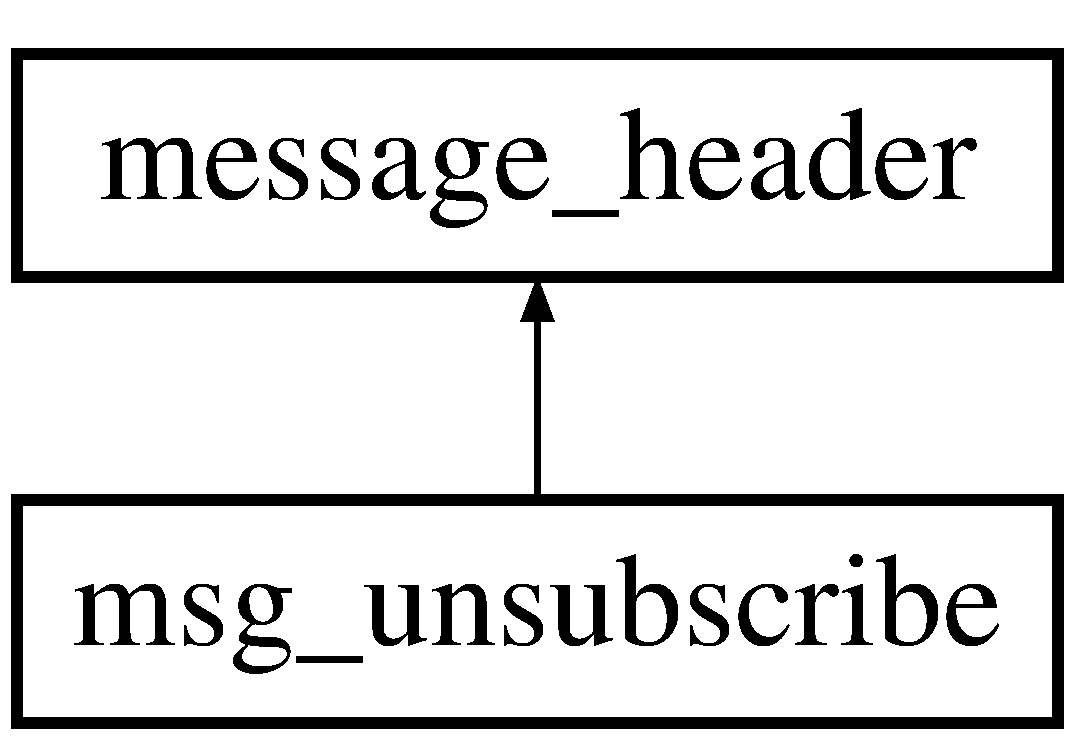
\includegraphics[height=2.000000cm]{structmsg__unsubscribe}
\end{center}
\end{figure}
\subsection*{Public Attributes}
\begin{DoxyCompactItemize}
\item 
\hypertarget{structmsg__unsubscribe_ae4b2ad5d8ea5604db234c60102c39ceb}{uint8\-\_\-t {\bfseries flags}}\label{structmsg__unsubscribe_ae4b2ad5d8ea5604db234c60102c39ceb}

\item 
\hypertarget{structmsg__unsubscribe_acbeb42e6a11b7cd265e6ef7ebf3aaf12}{uint16\-\_\-t {\bfseries message\-\_\-id}}\label{structmsg__unsubscribe_acbeb42e6a11b7cd265e6ef7ebf3aaf12}

\item 
\hypertarget{structmsg__unsubscribe_a424c2195d67a9afe4b8fc9e96baff5c4}{\begin{tabbing}
xx\=xx\=xx\=xx\=xx\=xx\=xx\=xx\=xx\=\kill
union \{\\
\hypertarget{unionmsg__unsubscribe_1_1@2_a5350896c7167af4b519c16e1f7af4694}{\>char {\bfseries topic\_name} \mbox{[}0\mbox{]}\\
\hypertarget{unionmsg__unsubscribe_1_1@2_a25d56e53c421a912f147125208b8c834}{\>uint16\_t {\bfseries topic\_id}\\
\}; }\label{structmsg__unsubscribe_a424c2195d67a9afe4b8fc9e96baff5c4}
\\

\end{tabbing}\end{DoxyCompactItemize}


The documentation for this struct was generated from the following file\-:\begin{DoxyCompactItemize}
\item 
\hyperlink{thing__defines_8h}{thing\-\_\-defines.\-h}\end{DoxyCompactItemize}

\hypertarget{structmsg__willmsg}{\section{msg\-\_\-willmsg Struct Reference}
\label{structmsg__willmsg}\index{msg\-\_\-willmsg@{msg\-\_\-willmsg}}
}
Inheritance diagram for msg\-\_\-willmsg\-:\begin{figure}[H]
\begin{center}
\leavevmode
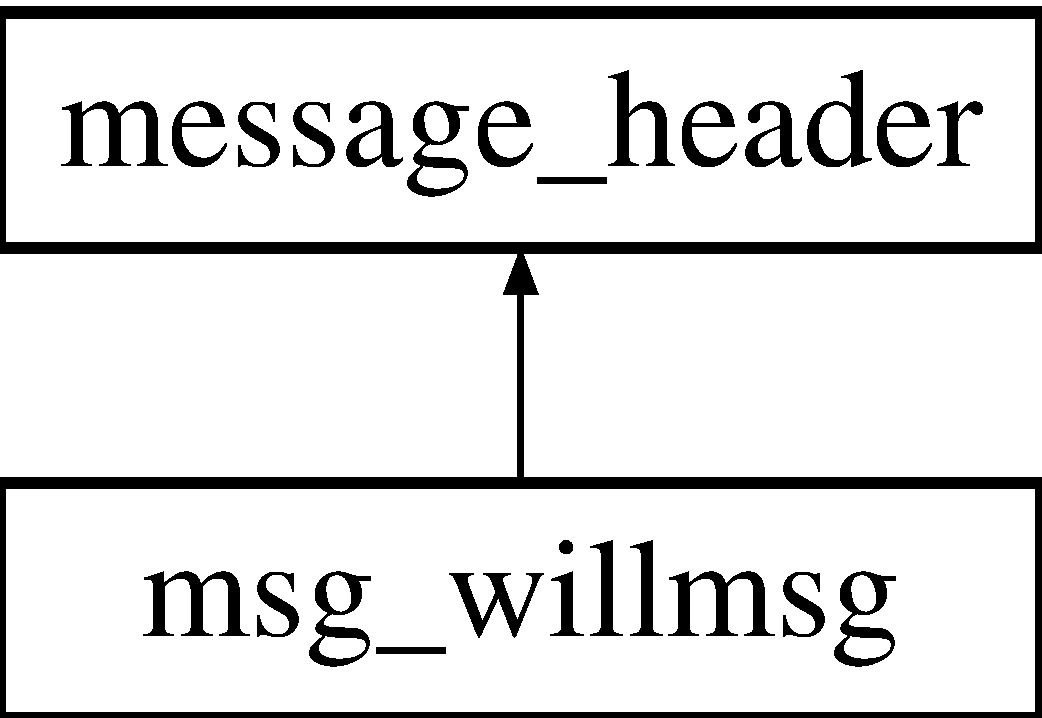
\includegraphics[height=2.000000cm]{structmsg__willmsg}
\end{center}
\end{figure}
\subsection*{Public Attributes}
\begin{DoxyCompactItemize}
\item 
\hypertarget{structmsg__willmsg_abfa8a96974590708e5c7264f3cd5f725}{char {\bfseries willmsg} \mbox{[}0\mbox{]}}\label{structmsg__willmsg_abfa8a96974590708e5c7264f3cd5f725}

\end{DoxyCompactItemize}


The documentation for this struct was generated from the following file\-:\begin{DoxyCompactItemize}
\item 
\hyperlink{thing__defines_8h}{thing\-\_\-defines.\-h}\end{DoxyCompactItemize}

\hypertarget{structmsg__willmsgresp}{\section{msg\-\_\-willmsgresp Struct Reference}
\label{structmsg__willmsgresp}\index{msg\-\_\-willmsgresp@{msg\-\_\-willmsgresp}}
}
Inheritance diagram for msg\-\_\-willmsgresp\-:\begin{figure}[H]
\begin{center}
\leavevmode
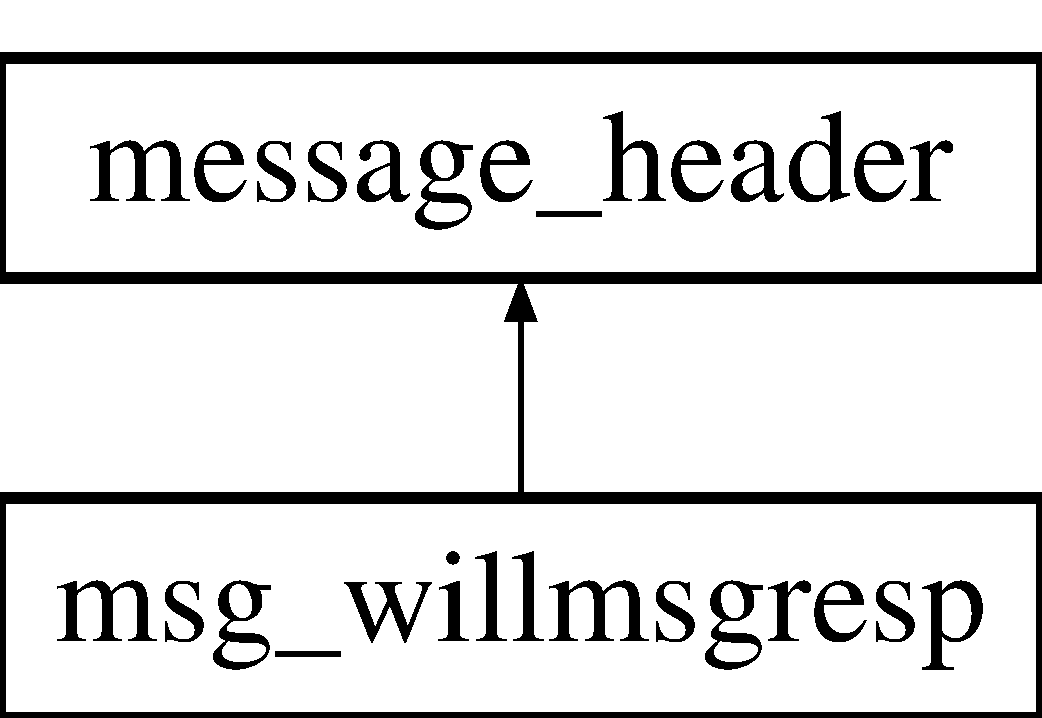
\includegraphics[height=2.000000cm]{structmsg__willmsgresp}
\end{center}
\end{figure}
\subsection*{Public Attributes}
\begin{DoxyCompactItemize}
\item 
\hypertarget{structmsg__willmsgresp_abe4556de0f72082d28f175e39681fb98}{uint8\-\_\-t {\bfseries return\-\_\-code}}\label{structmsg__willmsgresp_abe4556de0f72082d28f175e39681fb98}

\end{DoxyCompactItemize}


The documentation for this struct was generated from the following file\-:\begin{DoxyCompactItemize}
\item 
\hyperlink{thing__defines_8h}{thing\-\_\-defines.\-h}\end{DoxyCompactItemize}

\hypertarget{structmsg__willtopic}{\section{msg\-\_\-willtopic Struct Reference}
\label{structmsg__willtopic}\index{msg\-\_\-willtopic@{msg\-\_\-willtopic}}
}
Inheritance diagram for msg\-\_\-willtopic\-:\begin{figure}[H]
\begin{center}
\leavevmode
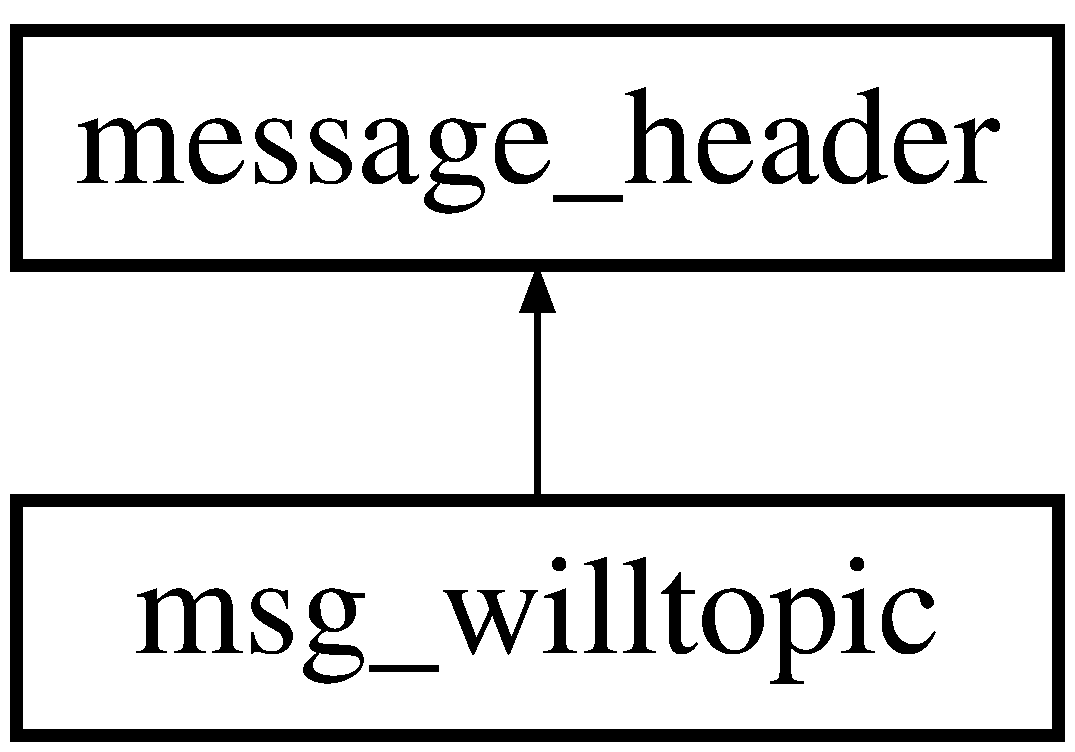
\includegraphics[height=2.000000cm]{structmsg__willtopic}
\end{center}
\end{figure}
\subsection*{Public Attributes}
\begin{DoxyCompactItemize}
\item 
\hypertarget{structmsg__willtopic_a5237e6b07977b4136bacfa87556c6acd}{uint8\-\_\-t {\bfseries flags}}\label{structmsg__willtopic_a5237e6b07977b4136bacfa87556c6acd}

\item 
\hypertarget{structmsg__willtopic_a5814f73f2d1c453f99f1ccd8fc955d6d}{char {\bfseries will\-\_\-topic} \mbox{[}0\mbox{]}}\label{structmsg__willtopic_a5814f73f2d1c453f99f1ccd8fc955d6d}

\end{DoxyCompactItemize}


The documentation for this struct was generated from the following file\-:\begin{DoxyCompactItemize}
\item 
\hyperlink{thing__defines_8h}{thing\-\_\-defines.\-h}\end{DoxyCompactItemize}

\hypertarget{structmsg__willtopicresp}{\section{msg\-\_\-willtopicresp Struct Reference}
\label{structmsg__willtopicresp}\index{msg\-\_\-willtopicresp@{msg\-\_\-willtopicresp}}
}
Inheritance diagram for msg\-\_\-willtopicresp\-:\begin{figure}[H]
\begin{center}
\leavevmode
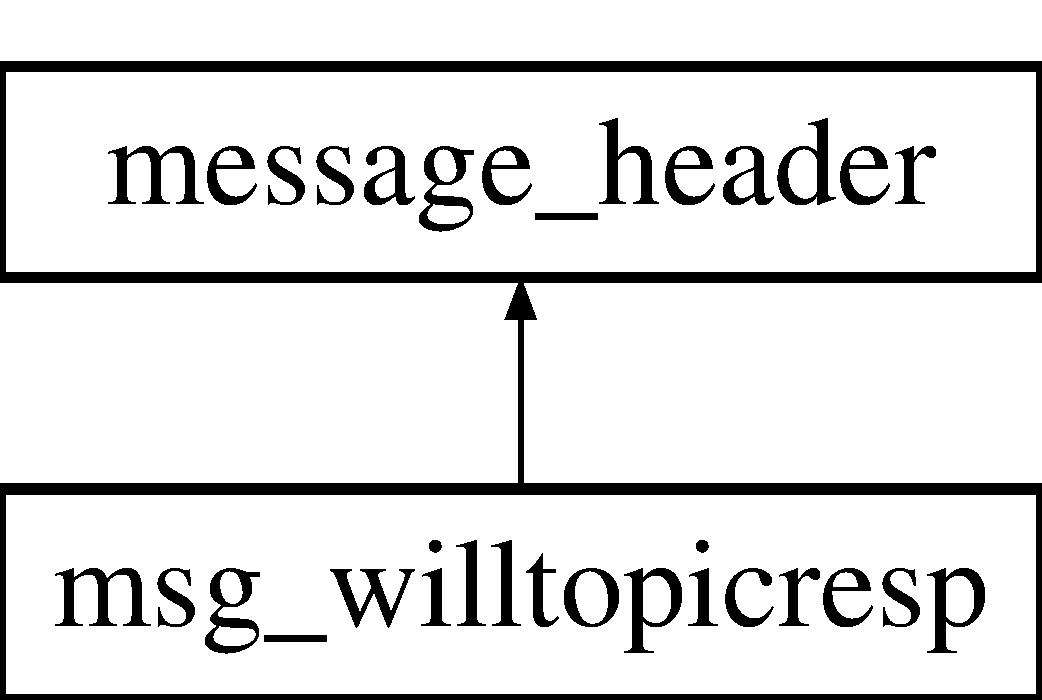
\includegraphics[height=2.000000cm]{structmsg__willtopicresp}
\end{center}
\end{figure}
\subsection*{Public Attributes}
\begin{DoxyCompactItemize}
\item 
\hypertarget{structmsg__willtopicresp_a0c5dc5afe02d246a3c657d258a47ead9}{uint8\-\_\-t {\bfseries return\-\_\-code}}\label{structmsg__willtopicresp_a0c5dc5afe02d246a3c657d258a47ead9}

\end{DoxyCompactItemize}


The documentation for this struct was generated from the following file\-:\begin{DoxyCompactItemize}
\item 
\hyperlink{thing__defines_8h}{thing\-\_\-defines.\-h}\end{DoxyCompactItemize}

\hypertarget{classThingClient}{\section{Thing\-Client Class Reference}
\label{classThingClient}\index{Thing\-Client@{Thing\-Client}}
}


A class for communication between thing and gateway.  




{\ttfamily \#include $<$thing\-\_\-client.\-h$>$}

\subsection*{Public Member Functions}
\begin{DoxyCompactItemize}
\item 
\hyperlink{classThingClient_a771f683ab76f89a2b22c85a5647df1e3}{Thing\-Client} (const char $\ast$id, Stream \&serial)
\item 
\hypertarget{classThingClient_a4f21f41869c7b1e01c62ef7939b247b5}{void {\bfseries Add} (\hyperlink{classCapitalValue}{Capital\-Value} \&v)}\label{classThingClient_a4f21f41869c7b1e01c62ef7939b247b5}

\item 
\hypertarget{classThingClient_ab2f23f07a087ef56bd57cdf77bac9b4f}{void {\bfseries Add} (\hyperlink{classCapitalFunction}{Capital\-Function} \&f)}\label{classThingClient_ab2f23f07a087ef56bd57cdf77bac9b4f}

\item 
void \hyperlink{classThingClient_aedab0c0ee3c96530eb6beed1f2a459b6}{set\-\_\-serial} (Stream \&serial)
\item 
void \hyperlink{classThingClient_afbfe83248b51bbbf484d19c11e8202a7}{set\-\_\-connect\-\_\-handler} (void($\ast$connect\-Handler)())
\item 
void \hyperlink{classThingClient_a598656f81507d9e295149379a06d6cbc}{set\-\_\-disconnect\-\_\-handler} (void($\ast$disconnect\-Handler)())
\item 
\hypertarget{classThingClient_a61c3913c2a50be164e9a239d1ac42363}{void {\bfseries set\-\_\-client\-\_\-id} (const char $\ast$id)}\label{classThingClient_a61c3913c2a50be164e9a239d1ac42363}

\item 
void \hyperlink{classThingClient_a9afef6f565bd4277939406ef6a324bfe}{Setting} ()
\item 
void \hyperlink{classThingClient_a27695ee5231952c6aa1d9431b1ea884d}{Do\-Loop} (int pub\-\_\-period=100)
\end{DoxyCompactItemize}
\subsection*{Protected Member Functions}
\begin{DoxyCompactItemize}
\item 
\hypertarget{classThingClient_a7c3221f6d72ce2e47a783a0815171345}{virtual void {\bfseries pingreq\-Handler} ()}\label{classThingClient_a7c3221f6d72ce2e47a783a0815171345}

\item 
\hypertarget{classThingClient_ac4ab103343209f93a0cbeab0d5761a1c}{virtual void {\bfseries pingresp\-Handler} ()}\label{classThingClient_ac4ab103343209f93a0cbeab0d5761a1c}

\item 
\hypertarget{classThingClient_ac66bac1316dfe88086278835cca1e1d2}{virtual void {\bfseries suback\-Handler} (const \hyperlink{structmsg__suback}{msg\-\_\-suback} $\ast$msg)}\label{classThingClient_ac66bac1316dfe88086278835cca1e1d2}

\item 
\hypertarget{classThingClient_ab807f216f8c25cd40800959ebec71dab}{virtual void {\bfseries disconnect\-Handler} (const \hyperlink{structmsg__disconnect}{msg\-\_\-disconnect} $\ast$msg)}\label{classThingClient_ab807f216f8c25cd40800959ebec71dab}

\item 
\hypertarget{classThingClient_ab8bc8252846e50800c5dc0543e7b0309}{void {\bfseries regack} (const uint16\-\_\-t topic\-Id, const uint16\-\_\-t message\-Id, const return\-\_\-code\-\_\-t return\-\_\-code)}\label{classThingClient_ab8bc8252846e50800c5dc0543e7b0309}

\item 
\hypertarget{classThingClient_aca0d151dc7fafd12c564810a4a57d353}{void {\bfseries puback} (const uint16\-\_\-t topic\-Id, const uint16\-\_\-t message\-Id, const return\-\_\-code\-\_\-t return\-\_\-code)}\label{classThingClient_aca0d151dc7fafd12c564810a4a57d353}

\item 
\hypertarget{classThingClient_a672b424a4c7db25c6c9c851ab65688a3}{void {\bfseries subscribe} (const uint8\-\_\-t flags, const uint16\-\_\-t topic\-Id)}\label{classThingClient_a672b424a4c7db25c6c9c851ab65688a3}

\item 
\hypertarget{classThingClient_a3c0f6a25ffa7b1cfa5c17b82a4b1125b}{void {\bfseries unsubscribe} (const uint8\-\_\-t flags, const uint16\-\_\-t topic\-Id)}\label{classThingClient_a3c0f6a25ffa7b1cfa5c17b82a4b1125b}

\item 
\hypertarget{classThingClient_a0b2105ce5421f8859664cac4b32e6478}{void {\bfseries devreg\-Handler} ()}\label{classThingClient_a0b2105ce5421f8859664cac4b32e6478}

\item 
\hypertarget{classThingClient_ad627f7e69476311017ef903144d6a505}{void {\bfseries devregack\-Handler} (const \hyperlink{structmsg__devregack}{msg\-\_\-devregack} $\ast$msg)}\label{classThingClient_ad627f7e69476311017ef903144d6a505}

\item 
\hypertarget{classThingClient_a08b89371ea7017864a53e4973109a178}{void {\bfseries regack\-Handler} (const \hyperlink{structmsg__regack}{msg\-\_\-regack} $\ast$msg)}\label{classThingClient_a08b89371ea7017864a53e4973109a178}

\item 
\hypertarget{classThingClient_acc74fdf4e099d0e9bb8ca4b5c431b11a}{void {\bfseries publish\-Handler} (const \hyperlink{structmsg__publish}{msg\-\_\-publish} $\ast$msg)}\label{classThingClient_acc74fdf4e099d0e9bb8ca4b5c431b11a}

\item 
\hypertarget{classThingClient_aa99dbe36483893c9c68533f1f6f037ab}{void {\bfseries advertise\-Handler} (const \hyperlink{structmsg__advertise}{msg\-\_\-advertise} $\ast$msg)}\label{classThingClient_aa99dbe36483893c9c68533f1f6f037ab}

\item 
\hypertarget{classThingClient_a2080616403d90b82f2ccf64198c8c156}{void {\bfseries gwinfo\-Handler} (const \hyperlink{structmsg__gwinfo}{msg\-\_\-gwinfo} $\ast$msg)}\label{classThingClient_a2080616403d90b82f2ccf64198c8c156}

\item 
\hypertarget{classThingClient_a6a460a7dc9e59e39fe6e3c25b742281a}{void {\bfseries connack\-Handler} (const \hyperlink{structmsg__connack}{msg\-\_\-connack} $\ast$msg)}\label{classThingClient_a6a460a7dc9e59e39fe6e3c25b742281a}

\end{DoxyCompactItemize}


\subsection{Detailed Description}
A class for communication between thing and gateway. 

A programmer should declare this class and set id, set serial, add values and functions. then call .Setting on setting tab, and Publish in loop(). it acts like as a bridge between thing and middleware. it is very similar to the Class Client in thing\-\_\-client. please refer that documentation. 

\subsection{Constructor \& Destructor Documentation}
\hypertarget{classThingClient_a771f683ab76f89a2b22c85a5647df1e3}{\index{Thing\-Client@{Thing\-Client}!Thing\-Client@{Thing\-Client}}
\index{Thing\-Client@{Thing\-Client}!ThingClient@{Thing\-Client}}
\subsubsection[{Thing\-Client}]{\setlength{\rightskip}{0pt plus 5cm}Thing\-Client\-::\-Thing\-Client (
\begin{DoxyParamCaption}
\item[{const char $\ast$}]{id, }
\item[{Stream \&}]{serial}
\end{DoxyParamCaption}
)}}\label{classThingClient_a771f683ab76f89a2b22c85a5647df1e3}
programmer can easily set client id and zigbee serial with this constructor. 

\subsection{Member Function Documentation}
\hypertarget{classThingClient_a27695ee5231952c6aa1d9431b1ea884d}{\index{Thing\-Client@{Thing\-Client}!Do\-Loop@{Do\-Loop}}
\index{Do\-Loop@{Do\-Loop}!ThingClient@{Thing\-Client}}
\subsubsection[{Do\-Loop}]{\setlength{\rightskip}{0pt plus 5cm}void Thing\-Client\-::\-Do\-Loop (
\begin{DoxyParamCaption}
\item[{int}]{pub\-\_\-period = {\ttfamily 100}}
\end{DoxyParamCaption}
)}}\label{classThingClient_a27695ee5231952c6aa1d9431b1ea884d}
Call it in the loop() tab on Arduino I\-D\-E Environment. \hypertarget{classThingClient_afbfe83248b51bbbf484d19c11e8202a7}{\index{Thing\-Client@{Thing\-Client}!set\-\_\-connect\-\_\-handler@{set\-\_\-connect\-\_\-handler}}
\index{set\-\_\-connect\-\_\-handler@{set\-\_\-connect\-\_\-handler}!ThingClient@{Thing\-Client}}
\subsubsection[{set\-\_\-connect\-\_\-handler}]{\setlength{\rightskip}{0pt plus 5cm}void Thing\-Client\-::set\-\_\-connect\-\_\-handler (
\begin{DoxyParamCaption}
\item[{void($\ast$)()}]{connect\-Handler}
\end{DoxyParamCaption}
)}}\label{classThingClient_afbfe83248b51bbbf484d19c11e8202a7}
set function that acts when arduino connects to the gateway 
\begin{DoxyParams}{Parameters}
{\em connect\-Handler} & the void function that programmer wants to activate when arduino connects to the gateway. \\
\hline
\end{DoxyParams}
\hypertarget{classThingClient_a598656f81507d9e295149379a06d6cbc}{\index{Thing\-Client@{Thing\-Client}!set\-\_\-disconnect\-\_\-handler@{set\-\_\-disconnect\-\_\-handler}}
\index{set\-\_\-disconnect\-\_\-handler@{set\-\_\-disconnect\-\_\-handler}!ThingClient@{Thing\-Client}}
\subsubsection[{set\-\_\-disconnect\-\_\-handler}]{\setlength{\rightskip}{0pt plus 5cm}void Thing\-Client\-::set\-\_\-disconnect\-\_\-handler (
\begin{DoxyParamCaption}
\item[{void($\ast$)()}]{disconnect\-Handler}
\end{DoxyParamCaption}
)}}\label{classThingClient_a598656f81507d9e295149379a06d6cbc}
set function that acts when arduino disconnects from the gateway 
\begin{DoxyParams}{Parameters}
{\em disconnect\-Handler} & the void function that programmer wants to activate when arduino disconnects from the gateway. \\
\hline
\end{DoxyParams}
\hypertarget{classThingClient_aedab0c0ee3c96530eb6beed1f2a459b6}{\index{Thing\-Client@{Thing\-Client}!set\-\_\-serial@{set\-\_\-serial}}
\index{set\-\_\-serial@{set\-\_\-serial}!ThingClient@{Thing\-Client}}
\subsubsection[{set\-\_\-serial}]{\setlength{\rightskip}{0pt plus 5cm}void Thing\-Client\-::set\-\_\-serial (
\begin{DoxyParamCaption}
\item[{Stream \&}]{serial}
\end{DoxyParamCaption}
)}}\label{classThingClient_aedab0c0ee3c96530eb6beed1f2a459b6}
set serial that connected to the zigbee output and input \hypertarget{classThingClient_a9afef6f565bd4277939406ef6a324bfe}{\index{Thing\-Client@{Thing\-Client}!Setting@{Setting}}
\index{Setting@{Setting}!ThingClient@{Thing\-Client}}
\subsubsection[{Setting}]{\setlength{\rightskip}{0pt plus 5cm}void Thing\-Client\-::\-Setting (
\begin{DoxyParamCaption}
{}
\end{DoxyParamCaption}
)}}\label{classThingClient_a9afef6f565bd4277939406ef6a324bfe}
Call it after setting serial, setting client id, and Adding every function and value. Do not forget call this function after (zigbee serial).begin(9600)! it should be called in the setting() tab on Arduino I\-D\-E Environment. 

The documentation for this class was generated from the following files\-:\begin{DoxyCompactItemize}
\item 
\hyperlink{thing__client_8h}{thing\-\_\-client.\-h}\item 
thing\-\_\-client.\-cpp\end{DoxyCompactItemize}

\chapter{File Documentation}
\hypertarget{thing__client_8h}{\section{thing\-\_\-client.\-h File Reference}
\label{thing__client_8h}\index{thing\-\_\-client.\-h@{thing\-\_\-client.\-h}}
}


class Value, Function, Client included  


{\ttfamily \#include $<$Arduino.\-h$>$}\\*
{\ttfamily \#include $<$Stream.\-h$>$}\\*
{\ttfamily \#include \char`\"{}Software\-Serial/\-Software\-Serial.\-h\char`\"{}}\\*
{\ttfamily \#include \char`\"{}../\-X\-Bee/\-X\-Bee.\-h\char`\"{}}\\*
{\ttfamily \#include \char`\"{}thing\-\_\-defines.\-h\char`\"{}}\\*
\subsection*{Classes}
\begin{DoxyCompactItemize}
\item 
class \hyperlink{classCapitalValue}{Capital\-Value}
\begin{DoxyCompactList}\small\item\em A class for handling various \char`\"{}value\char`\"{} types. \end{DoxyCompactList}\item 
class \hyperlink{classCapitalFunction}{Capital\-Function}
\begin{DoxyCompactList}\small\item\em A class for handling various \char`\"{}function\char`\"{} types. \end{DoxyCompactList}\item 
class \hyperlink{classThingClient}{Thing\-Client}
\begin{DoxyCompactList}\small\item\em A class for communication between thing and gateway. \end{DoxyCompactList}\end{DoxyCompactItemize}
\subsection*{Macros}
\begin{DoxyCompactItemize}
\item 
\hypertarget{thing__client_8h_ad65394f97c514e8ee5587f441cda85c5}{\#define {\bfseries C\-A\-P\-I\-T\-A\-L\-\_\-\-M\-A\-X\-\_\-\-V\-A\-L\-U\-E}~5}\label{thing__client_8h_ad65394f97c514e8ee5587f441cda85c5}

\item 
\hypertarget{thing__client_8h_a92b5ef6232f0c8bc5da2167fec7a43d9}{\#define {\bfseries C\-A\-P\-I\-T\-A\-L\-\_\-\-M\-A\-X\-\_\-\-F\-U\-N\-C\-T\-I\-O\-N}~3}\label{thing__client_8h_a92b5ef6232f0c8bc5da2167fec7a43d9}

\item 
\hypertarget{thing__client_8h_a2e2abe162d63ff25886d5397953e1c85}{\#define {\bfseries C\-A\-P\-I\-T\-A\-L\-\_\-\-M\-A\-X\-\_\-\-N\-A\-M\-E\-\_\-\-L\-E\-N\-G\-T\-H}~11}\label{thing__client_8h_a2e2abe162d63ff25886d5397953e1c85}

\item 
\hypertarget{thing__client_8h_aeb20094cdd1fcb48dc040a5bb94345d0}{\#define {\bfseries C\-A\-P\-I\-T\-A\-L\-\_\-\-M\-A\-X\-\_\-\-B\-U\-F\-F\-E\-R\-\_\-\-S\-I\-Z\-E}~55}\label{thing__client_8h_aeb20094cdd1fcb48dc040a5bb94345d0}

\end{DoxyCompactItemize}


\subsection{Detailed Description}
class Value, Function, Client included \begin{DoxyAuthor}{Author}
Donghyun Kang, \href{mailto:kangdongh@iris.snu.ac.kr}{\tt kangdongh@iris.\-snu.\-ac.\-kr} 
\end{DoxyAuthor}
\begin{DoxyDate}{Date}
2016-\/04-\/01 
\end{DoxyDate}
\begin{DoxyVersion}{Version}
1.\-0.\-0 
\end{DoxyVersion}
\hypertarget{thing__client_8h_changelog}{}\subsection{Change Log}\label{thing__client_8h_changelog}
2016/04/01 the first reconstruction applied \hypertarget{thing__client_8h_license_section}{}\subsection{License}\label{thing__client_8h_license_section}
T\-O\-D\-O 
\hypertarget{thing__defines_8h}{\section{thing\-\_\-defines.\-h File Reference}
\label{thing__defines_8h}\index{thing\-\_\-defines.\-h@{thing\-\_\-defines.\-h}}
}


define macros, default enums and types  


\subsection*{Classes}
\begin{DoxyCompactItemize}
\item 
union \hyperlink{union__cvalue}{\-\_\-cvalue}
\item 
struct \hyperlink{structmessage__header}{message\-\_\-header}
\item 
struct \hyperlink{structmsg__advertise}{msg\-\_\-advertise}
\item 
struct \hyperlink{structmsg__searchgw}{msg\-\_\-searchgw}
\item 
struct \hyperlink{structmsg__gwinfo}{msg\-\_\-gwinfo}
\item 
struct \hyperlink{structmsg__connect}{msg\-\_\-connect}
\item 
struct \hyperlink{structmsg__connack}{msg\-\_\-connack}
\item 
struct \hyperlink{structmsg__willtopic}{msg\-\_\-willtopic}
\item 
struct \hyperlink{structmsg__willmsg}{msg\-\_\-willmsg}
\item 
struct \hyperlink{structmsg__register}{msg\-\_\-register}
\item 
struct \hyperlink{structmsg__regack}{msg\-\_\-regack}
\item 
struct \hyperlink{structmsg__publish}{msg\-\_\-publish}
\item 
struct \hyperlink{structmsg__puback}{msg\-\_\-puback}
\item 
struct \hyperlink{structmsg__pubqos2}{msg\-\_\-pubqos2}
\item 
struct \hyperlink{structmsg__subscribe}{msg\-\_\-subscribe}
\item 
struct \hyperlink{structmsg__suback}{msg\-\_\-suback}
\item 
struct \hyperlink{structmsg__devreg}{msg\-\_\-devreg}
\item 
struct \hyperlink{structmsg__devregack}{msg\-\_\-devregack}
\item 
struct \hyperlink{structmsg__unsubscribe}{msg\-\_\-unsubscribe}
\item 
struct \hyperlink{structmsg__unsuback}{msg\-\_\-unsuback}
\item 
struct \hyperlink{structmsg__pingreq}{msg\-\_\-pingreq}
\item 
struct \hyperlink{structmsg__disconnect}{msg\-\_\-disconnect}
\item 
struct \hyperlink{structmsg__willtopicresp}{msg\-\_\-willtopicresp}
\item 
struct \hyperlink{structmsg__willmsgresp}{msg\-\_\-willmsgresp}
\end{DoxyCompactItemize}
\subsection*{Macros}
\begin{DoxyCompactItemize}
\item 
\hypertarget{thing__defines_8h_af06c4fd66ec27510cb5937fe6c3e224f}{\#define {\bfseries C\-O\-M\-M\-O\-N0000}~\char`\"{}\%s/\%s\char`\"{}}\label{thing__defines_8h_af06c4fd66ec27510cb5937fe6c3e224f}

\item 
\hypertarget{thing__defines_8h_a739930c33dd8dbd78b1219f7c4733f1f}{\#define {\bfseries M\-T1001}~\char`\"{}M\-T/R\-E\-G\-A\-C\-K/\%s\char`\"{}}\label{thing__defines_8h_a739930c33dd8dbd78b1219f7c4733f1f}

\item 
\hypertarget{thing__defines_8h_a35bd0a7424b3fc32391f0b16de083c6d}{\#define {\bfseries M\-T1002}~\char`\"{}M\-T/P\-I\-N\-G\-R\-E\-Q/\%s\char`\"{}}\label{thing__defines_8h_a35bd0a7424b3fc32391f0b16de083c6d}

\item 
\hypertarget{thing__defines_8h_a5ddad194951a166a740fa4edb76f993e}{\#define {\bfseries M\-T1003}~\char`\"{}M\-T/\%s/\%s\char`\"{}}\label{thing__defines_8h_a5ddad194951a166a740fa4edb76f993e}

\item 
\hypertarget{thing__defines_8h_a69c2784847a0191061c9e92970b85390}{\#define {\bfseries T\-M2001}~\char`\"{}T\-M/R\-E\-G\-I\-S\-T\-E\-R/\%s\char`\"{}}\label{thing__defines_8h_a69c2784847a0191061c9e92970b85390}

\item 
\hypertarget{thing__defines_8h_a1c0b45ae33aeebfe72890b8f424205d5}{\#define {\bfseries T\-M2002}~\char`\"{}T\-M/U\-N\-R\-E\-G\-I\-S\-T\-E\-R/\%s\char`\"{}}\label{thing__defines_8h_a1c0b45ae33aeebfe72890b8f424205d5}

\item 
\hypertarget{thing__defines_8h_afc98b679a68c2a4c5c6a52154e084691}{\#define {\bfseries T\-M2003}~\char`\"{}T\-M/P\-I\-N\-G\-R\-E\-S\-P/\%s\char`\"{}}\label{thing__defines_8h_afc98b679a68c2a4c5c6a52154e084691}

\item 
\hypertarget{thing__defines_8h_a4792dca6ae311df86f1c5339d9f22410}{\#define {\bfseries T\-M2004}~\char`\"{}T\-M/R\-E\-S\-U\-L\-T/F\-U\-N\-C\-T\-I\-O\-N/\%s\char`\"{}}\label{thing__defines_8h_a4792dca6ae311df86f1c5339d9f22410}

\item 
\hypertarget{thing__defines_8h_a1e5759eb3f87b00bf4acf6579f9034d5}{\#define {\bfseries Q\-O\-S}~2}\label{thing__defines_8h_a1e5759eb3f87b00bf4acf6579f9034d5}

\item 
\hypertarget{thing__defines_8h_a45ba202b05caf39795aeca91b0ae547e}{\#define {\bfseries T\-I\-M\-E\-O\-U\-T}~10000\-L}\label{thing__defines_8h_a45ba202b05caf39795aeca91b0ae547e}

\item 
\hypertarget{thing__defines_8h_ab7054d074aeaa58b41773e6a8e53ed8c}{\#define {\bfseries P\-R\-O\-T\-O\-C\-O\-L\-\_\-\-I\-D}~0x01}\label{thing__defines_8h_ab7054d074aeaa58b41773e6a8e53ed8c}

\item 
\hypertarget{thing__defines_8h_a3261e883d3252a2de00a0e4250f51407}{\#define {\bfseries F\-L\-A\-G\-\_\-\-D\-U\-P}~0x80}\label{thing__defines_8h_a3261e883d3252a2de00a0e4250f51407}

\item 
\hypertarget{thing__defines_8h_a6403d94bfd166a78b379fb365e4a45d3}{\#define {\bfseries F\-L\-A\-G\-\_\-\-Q\-O\-S\-\_\-0}~0x00}\label{thing__defines_8h_a6403d94bfd166a78b379fb365e4a45d3}

\item 
\hypertarget{thing__defines_8h_a97e12e0479112450e1eabba068b46314}{\#define {\bfseries F\-L\-A\-G\-\_\-\-Q\-O\-S\-\_\-1}~0x20}\label{thing__defines_8h_a97e12e0479112450e1eabba068b46314}

\item 
\hypertarget{thing__defines_8h_ab9615bfbde2553636a2f274f0a7735c1}{\#define {\bfseries F\-L\-A\-G\-\_\-\-Q\-O\-S\-\_\-2}~0x40}\label{thing__defines_8h_ab9615bfbde2553636a2f274f0a7735c1}

\item 
\hypertarget{thing__defines_8h_a2a043e7a2b30617ca8e614da1da88cc5}{\#define {\bfseries F\-L\-A\-G\-\_\-\-Q\-O\-S\-\_\-\-M1}~0x60}\label{thing__defines_8h_a2a043e7a2b30617ca8e614da1da88cc5}

\item 
\hypertarget{thing__defines_8h_a2f2024b544e12b3ef3327fd2c897d890}{\#define {\bfseries F\-L\-A\-G\-\_\-\-R\-E\-T\-A\-I\-N}~0x10}\label{thing__defines_8h_a2f2024b544e12b3ef3327fd2c897d890}

\item 
\hypertarget{thing__defines_8h_a5c3b06ba7a0ce1121e869bafcbfde509}{\#define {\bfseries F\-L\-A\-G\-\_\-\-W\-I\-L\-L}~0x08}\label{thing__defines_8h_a5c3b06ba7a0ce1121e869bafcbfde509}

\item 
\hypertarget{thing__defines_8h_a46dcd33ac11d789ca7079b1ea798f340}{\#define {\bfseries F\-L\-A\-G\-\_\-\-C\-L\-E\-A\-N}~0x04}\label{thing__defines_8h_a46dcd33ac11d789ca7079b1ea798f340}

\item 
\hypertarget{thing__defines_8h_a291a223782cf21ff551ba2fa3aee1df9}{\#define {\bfseries F\-L\-A\-G\-\_\-\-T\-O\-P\-I\-C\-\_\-\-N\-A\-M\-E}~0x00}\label{thing__defines_8h_a291a223782cf21ff551ba2fa3aee1df9}

\item 
\hypertarget{thing__defines_8h_a5c5591db332e01da1b90b86d49e392b1}{\#define {\bfseries F\-L\-A\-G\-\_\-\-T\-O\-P\-I\-C\-\_\-\-P\-R\-E\-D\-E\-F\-I\-N\-E\-D\-\_\-\-I\-D}~0x01}\label{thing__defines_8h_a5c5591db332e01da1b90b86d49e392b1}

\item 
\hypertarget{thing__defines_8h_ade0c87f8533c839c2c0a13a81927c8ab}{\#define {\bfseries F\-L\-A\-G\-\_\-\-T\-O\-P\-I\-C\-\_\-\-S\-H\-O\-R\-T\-\_\-\-N\-A\-M\-E}~0x02}\label{thing__defines_8h_ade0c87f8533c839c2c0a13a81927c8ab}

\item 
\hypertarget{thing__defines_8h_a30e56823c3a44ca9ba12d24ca20c316c}{\#define {\bfseries Q\-O\-S\-\_\-\-M\-A\-S\-K}~(F\-L\-A\-G\-\_\-\-Q\-O\-S\-\_\-0 $\vert$ F\-L\-A\-G\-\_\-\-Q\-O\-S\-\_\-1 $\vert$ F\-L\-A\-G\-\_\-\-Q\-O\-S\-\_\-2 $\vert$ F\-L\-A\-G\-\_\-\-Q\-O\-S\-\_\-\-M1)}\label{thing__defines_8h_a30e56823c3a44ca9ba12d24ca20c316c}

\item 
\hypertarget{thing__defines_8h_a25b9f6533efd7b3caf52d7f873352234}{\#define {\bfseries T\-O\-P\-I\-C\-\_\-\-M\-A\-S\-K}~(F\-L\-A\-G\-\_\-\-T\-O\-P\-I\-C\-\_\-\-N\-A\-M\-E $\vert$ F\-L\-A\-G\-\_\-\-T\-O\-P\-I\-C\-\_\-\-P\-R\-E\-D\-E\-F\-I\-N\-E\-D\-\_\-\-I\-D $\vert$ F\-L\-A\-G\-\_\-\-T\-O\-P\-I\-C\-\_\-\-S\-H\-O\-R\-T\-\_\-\-N\-A\-M\-E)}\label{thing__defines_8h_a25b9f6533efd7b3caf52d7f873352234}

\item 
\hypertarget{thing__defines_8h_af9d487d4de32a0e7f0bc3c3927156812}{\#define {\bfseries T\-\_\-\-A\-D\-V}~960}\label{thing__defines_8h_af9d487d4de32a0e7f0bc3c3927156812}

\item 
\hypertarget{thing__defines_8h_a3bc2d3f926fc3741aab975705e9835c2}{\#define {\bfseries N\-\_\-\-A\-D\-V}~3}\label{thing__defines_8h_a3bc2d3f926fc3741aab975705e9835c2}

\item 
\hypertarget{thing__defines_8h_aaabbd824e56d98e3da47a7e101a5cf5d}{\#define {\bfseries T\-\_\-\-S\-E\-A\-R\-C\-H\-\_\-\-G\-W}~5}\label{thing__defines_8h_aaabbd824e56d98e3da47a7e101a5cf5d}

\item 
\hypertarget{thing__defines_8h_ac74429ed012d14cb0cd02dac322ad6fb}{\#define {\bfseries T\-\_\-\-G\-W\-\_\-\-I\-N\-F\-O}~5}\label{thing__defines_8h_ac74429ed012d14cb0cd02dac322ad6fb}

\item 
\hypertarget{thing__defines_8h_a54443be56482553ca412cf4c8ed89e6d}{\#define {\bfseries T\-\_\-\-W\-A\-I\-T}~360}\label{thing__defines_8h_a54443be56482553ca412cf4c8ed89e6d}

\item 
\hypertarget{thing__defines_8h_a285ac7b2259d61b6658e3a3710d171e1}{\#define {\bfseries T\-\_\-\-R\-E\-T\-R\-Y}~15}\label{thing__defines_8h_a285ac7b2259d61b6658e3a3710d171e1}

\item 
\hypertarget{thing__defines_8h_afaecd38e439e3849af73d2520736e697}{\#define {\bfseries N\-\_\-\-R\-E\-T\-R\-Y}~5}\label{thing__defines_8h_afaecd38e439e3849af73d2520736e697}

\item 
\hypertarget{thing__defines_8h_a16bd05079647d09c1999f7341ea5aa13}{\#define {\bfseries C\-A\-P\-\_\-\-D\-E\-B\-U\-G}}\label{thing__defines_8h_a16bd05079647d09c1999f7341ea5aa13}

\item 
\hypertarget{thing__defines_8h_a0189f26b96f87b4b28241be806116bd8}{\#define {\bfseries C\-P\-D\-B\-G}(...)~Serial.\-println(\-\_\-\-\_\-\-V\-A\-\_\-\-A\-R\-G\-S\-\_\-\-\_\-)}\label{thing__defines_8h_a0189f26b96f87b4b28241be806116bd8}

\item 
\hypertarget{thing__defines_8h_a61aed733f8e5502628b6a87e51ca4e4f}{\#define {\bfseries D\-O\-U\-B\-L\-E\-\_\-\-E\-P\-S\-I\-L\-O\-N}~(0.\-0000001)}\label{thing__defines_8h_a61aed733f8e5502628b6a87e51ca4e4f}

\item 
\hypertarget{thing__defines_8h_a653233c54662233137b6d4226244cca8}{\#define {\bfseries D\-O\-U\-B\-L\-E\-\_\-\-I\-S\-\_\-\-A\-P\-P\-R\-O\-X\-\_\-\-E\-Q\-U\-A\-L}(a, b)~(fabs((a) -\/ (b)) $<$= D\-O\-U\-B\-L\-E\-\_\-\-E\-P\-S\-I\-L\-O\-N)}\label{thing__defines_8h_a653233c54662233137b6d4226244cca8}

\end{DoxyCompactItemize}
\subsection*{Typedefs}
\begin{DoxyCompactItemize}
\item 
\hypertarget{thing__defines_8h_a1ec6f3cb761766b6d70f99b286155771}{typedef enum \-\_\-captype {\bfseries Cap\-Type}}\label{thing__defines_8h_a1ec6f3cb761766b6d70f99b286155771}

\item 
\hypertarget{thing__defines_8h_ad32d4699385a3311bf87a9968b57be43}{typedef enum \-\_\-capstate {\bfseries Cap\-State}}\label{thing__defines_8h_ad32d4699385a3311bf87a9968b57be43}

\item 
\hypertarget{thing__defines_8h_a53c5a1d25c860ffb13a235e42dee507a}{typedef union \hyperlink{union__cvalue}{\-\_\-cvalue} {\bfseries Cval}}\label{thing__defines_8h_a53c5a1d25c860ffb13a235e42dee507a}

\item 
\hypertarget{thing__defines_8h_abee737fbf33ca628e70a957ff7d23dff}{typedef void($\ast$ {\bfseries Void\-Function} )(void)}\label{thing__defines_8h_abee737fbf33ca628e70a957ff7d23dff}

\item 
\hypertarget{thing__defines_8h_a4f271344c3b9b5e743db98af0ebb102a}{typedef void($\ast$ {\bfseries Integer\-Function} )(int)}\label{thing__defines_8h_a4f271344c3b9b5e743db98af0ebb102a}

\item 
\hypertarget{thing__defines_8h_a974cab34c9250bd31cc896bee15a14a7}{typedef void($\ast$ {\bfseries Double\-Function} )(double)}\label{thing__defines_8h_a974cab34c9250bd31cc896bee15a14a7}

\item 
\hypertarget{thing__defines_8h_a80ca11a3c0322efc96585f8e8d73cf8a}{typedef void($\ast$ {\bfseries Bool\-Function} )(bool)}\label{thing__defines_8h_a80ca11a3c0322efc96585f8e8d73cf8a}

\item 
\hypertarget{thing__defines_8h_a6807f00dd1d49c9f95750ddb302f3d44}{typedef int($\ast$ {\bfseries Integer\-Value} )(void)}\label{thing__defines_8h_a6807f00dd1d49c9f95750ddb302f3d44}

\item 
\hypertarget{thing__defines_8h_ae9d4981d2ef4039771467c53897122aa}{typedef double($\ast$ {\bfseries Double\-Value} )(void)}\label{thing__defines_8h_ae9d4981d2ef4039771467c53897122aa}

\item 
\hypertarget{thing__defines_8h_a6dd8cd68910860eafb508179b1a9529f}{typedef bool($\ast$ {\bfseries Bool\-Value} )(void)}\label{thing__defines_8h_a6dd8cd68910860eafb508179b1a9529f}

\end{DoxyCompactItemize}
\subsection*{Enumerations}
\begin{DoxyCompactItemize}
\item 
enum {\bfseries \-\_\-captype} \{ \\*
{\bfseries U\-N\-D\-E\-F\-I\-N\-E\-D} = 0, 
{\bfseries V\-O\-I\-D}, 
{\bfseries I\-N\-T\-E\-G\-E\-R}, 
{\bfseries D\-O\-U\-B\-L\-E}, 
\\*
{\bfseries B\-O\-O\-L}
 \}
\item 
enum {\bfseries \-\_\-capstate} \{ {\bfseries U\-N\-R\-E\-G\-I\-S\-T\-E\-R\-E\-D} = 0, 
{\bfseries R\-E\-G\-I\-S\-T\-E\-R\-E\-D}
 \}
\item 
enum {\bfseries return\-\_\-code\-\_\-t} \{ {\bfseries A\-C\-C\-E\-P\-T\-E\-D}, 
{\bfseries R\-E\-J\-E\-C\-T\-E\-D\-\_\-\-C\-O\-N\-G\-E\-S\-T\-I\-O\-N}, 
{\bfseries R\-E\-J\-E\-C\-T\-E\-D\-\_\-\-I\-N\-V\-A\-L\-I\-D\-\_\-\-T\-O\-P\-I\-C\-\_\-\-I\-D}, 
{\bfseries R\-E\-J\-E\-C\-T\-E\-D\-\_\-\-N\-O\-T\-\_\-\-S\-U\-P\-P\-O\-R\-T\-E\-D}
 \}
\item 
enum {\bfseries message\-\_\-type} \{ \\*
{\bfseries A\-D\-V\-E\-R\-T\-I\-S\-E}, 
{\bfseries S\-E\-A\-R\-C\-H\-G\-W}, 
{\bfseries G\-W\-I\-N\-F\-O}, 
{\bfseries C\-O\-N\-N\-E\-C\-T} = 0x04, 
\\*
{\bfseries C\-O\-N\-N\-A\-C\-K}, 
{\bfseries W\-I\-L\-L\-T\-O\-P\-I\-C\-R\-E\-Q}, 
{\bfseries W\-I\-L\-L\-T\-O\-P\-I\-C}, 
{\bfseries W\-I\-L\-L\-M\-S\-G\-R\-E\-Q}, 
\\*
{\bfseries W\-I\-L\-L\-M\-S\-G}, 
{\bfseries R\-E\-G\-I\-S\-T\-E\-R}, 
{\bfseries R\-E\-G\-A\-C\-K}, 
{\bfseries P\-U\-B\-L\-I\-S\-H}, 
\\*
{\bfseries P\-U\-B\-A\-C\-K}, 
{\bfseries P\-U\-B\-C\-O\-M\-P}, 
{\bfseries P\-U\-B\-R\-E\-C}, 
{\bfseries P\-U\-B\-R\-E\-L}, 
\\*
{\bfseries S\-U\-B\-S\-C\-R\-I\-B\-E} = 0x12, 
{\bfseries S\-U\-B\-A\-C\-K}, 
{\bfseries U\-N\-S\-U\-B\-S\-C\-R\-I\-B\-E}, 
{\bfseries U\-N\-S\-U\-B\-A\-C\-K}, 
\\*
{\bfseries P\-I\-N\-G\-R\-E\-Q}, 
{\bfseries P\-I\-N\-G\-R\-E\-S\-P}, 
{\bfseries D\-I\-S\-C\-O\-N\-N\-E\-C\-T}, 
{\bfseries W\-I\-L\-L\-T\-O\-P\-I\-C\-U\-P\-D} = 0x1a, 
\\*
{\bfseries W\-I\-L\-L\-T\-O\-P\-I\-C\-R\-E\-S\-P}, 
{\bfseries W\-I\-L\-L\-M\-S\-G\-U\-P\-D}, 
{\bfseries W\-I\-L\-L\-M\-S\-G\-R\-E\-S\-P}, 
{\bfseries D\-E\-V\-R\-E\-G}, 
\\*
{\bfseries D\-E\-V\-R\-E\-G\-A\-C\-K}
 \}
\end{DoxyCompactItemize}


\subsection{Detailed Description}
define macros, default enums and types 
%--- End generated contents ---

% Index
\newpage
\phantomsection
\addcontentsline{toc}{chapter}{Index}
\printindex

\end{document}
